\documentclass[AMA,final,STIX1COL]{WileyNJD-v2}

\usepackage{xspace}
\usepackage{comment}
\usepackage{subfigure}
\articletype{Research Article}
\received{2 November, 2020}
\revised{TBD}
\accepted{TBD}

\raggedbottom

\def\COMPANION{{\scriptsize\url{https://gitlab.com/msserpa/prefetcher-ccpe}}\xspace}

\newcommand\new[1]{{\color{red}\textbf{#1}}}
\newcommand{\ms}[1]{\textcolor{orange}{\bfseries \ul{ msserpa: #1} }\vspace{0.2cm}}
\newcommand{\vsg}[1]{\textcolor{blue}{\bfseries \ul{vsgirelli: #1} }\vspace{0.2cm}}
\newcommand{\fbm}[1]{\textcolor{red}{\bfseries \ul{fbm: #1} }\vspace{0.2cm}}

\begin{document}

\title{Investigating Memory Prefetcher Performance over Parallel Applications: From Real to Simulated}

\author{Valéria S. Girelli*}
\author{Francis B. Moreira}
\author{Matheus S. Serpa}
\author{Danilo Carastan-Santos}
\author{Philippe O. A. Navaux}

\address{
  \orgdiv{Informatics Institute},
  \orgname{Federal University of Rio Grande do Sul -- UFRGS},
  \orgaddress{\city{Porto Alegre}, \country{Brazil}}}

\corres{*Valéria S. Girelli, UFRGS, Bento Gon\c{c}alves 9500, Porto Alegre -- RS, Brazil. \email{vsgirelli@inf.ufrgs.br}}

\authormark{Girelli \textsc{et al}}


\abstract[Summary]{
Memory prefetcher algorithms are widely used in processors to mitigate the performance gap between the processors and the memory subsystem. 
The complexities behind the architectures and prefetcher algorithms, however, not only hinder the development of accurate architecture simulators, but also hinder understanding the prefetcher's contribution to performance, on both a real hardware and in a simulated environment.
In this paper, we contribute to shed light the memory prefetcher's role in the performance of parallel HPC applications, considering the prefetcher algorithms offered by both the real hardware and the simulators. 
\new{We performed a careful experimental investigation}, executing the NAS parallel benchmark (NPB) on a real Skylake machine, and as well in a simulated environment with the ZSim and Sniper simulators, taking into account the prefetcher algorithms offered by both Skylake and the simulators. 
Our experimental results show that: (i) prefetching from the L3 to L2 cache presents better performance gains, (ii) the memory contention in the parallel execution constrains the prefetcher's effect, (iii) Skylake's parallel memory contention is poorly simulated by ZSim and Sniper, and (iv) Skylake's non-inclusive L3 cache hinders the accurate simulation of NPB with the Sniper's prefetchers.
}

\keywords{
computer architecture, 
parallel architecture, 
prefetcher, 
architecture simulation
}

\jnlcitation{\cname{
\author{V. S. Girelli},
\author{F. B. Moreira},
\author{M. S. Serpa},
\author{D. Carastan-Santos}, and
\author{P. O. A. Navaux}} (\cyear{2020}),
\ctitle{Investigating Memory Prefetcher Performance over Parallel Applications: From Real to Simulated},\cjournal{Concurrency and Computation: Practice and Experience}, \cvol{TBD}.}

\maketitle

\section{Introduction}\label{sec:introduction}

In recent years, there have been significant advances in the performance of processors, exemplified by the reduction of transistor size and the increase in the number of cores in a processor.
Conversely, the memory subsystem did not advance as significantly as processors, not being able to deliver data at the required rate. 
This problem is referred to in the literature as the memory wall~\cite{wulf1995memory}.
For this reason, there is a keen effort in computer architecture research to overcome these memory limitations. 
An example of a technology used to mitigate the memory latency is the prefetcher, a technique that identifies access patterns from each core, creates speculative memory requests, and fetches data -- that can be potentially useful -- to the cache beforehand.

In High-Performance Computing (HPC) systems, there are many other problems besides those inherent to the processors and memory individually. 
HPC applications are highly parallel, with many threads communicating with themselves, mainly through shared memory. For instance, (i) several threads access the same memory addresses, making necessary to keep data coherence in the several cache levels, and (ii) the memory interactions among different threads may also unpredictably change the data path through the memory hierarchy. 
When considering the memory hierarchy complexity of HPC systems along with the action of the prefetcher, the behavior of the processor's memory subsystem reaches a new level of complexity. 
The hindrance lies, therefore, in understanding how the prefetcher affects the processing performance of parallel, HPC applications.

To further complicate the matter, in computer architecture research, physical implementation and analysis are infeasible due to the high complexity and manufacturing costs. 
Consequently, architecture simulators are considered the primary mechanism to implement and evaluate new ideas~\cite{skadron2003challenges}, such as new prefetcher algorithms. 
To develop and analyze new ideas that attenuate problems arising from the inherent parallelism of HPC systems, we need multicore architecture simulators that support parallel workloads and accurately simulate interaction between cores.

In this work, we seek to shed light on the following questions: \textit{(i) how does the prefetcher affect the processing performance of parallel, HPC applications?}, and \textit{(ii) how can state-of-the-art architecture simulators accurately simulate HPC applications, with and without prefetcher?}

More specifically, this work presents the following set of contributions:
\begin{itemize}
    \item We developed a careful experimental investigation, executing the Numerical Aerodynamic Simulation Parallel Benchmark (NPB)~\cite{jin1999openmp};
    in an Intel Skylake machine and architecture simulations in the ZSim and Sniper simulators; 
    \item We show experimental evidence that an L2 memory prefetcher is more efficient in comparison with an L1 prefetcher, since avoiding excessive L3 cache accesses better contributes to performance, when comparing to accessing the L2 cache;
    \item We show evidence that the prefetchers' contribution to performance is limited by the level of parallelism of the application, mainly due to the increase in communication and memory contention as the level of parallelism increases;
    \item The Skylake and NPB simulation with ZSim and Sniper had poor accuracy in predicting the NPB applications performance, with and without simulating prefetcher algorithms, mainly due distinctions of the models and prefetcher algorithms present in ZSim and Sniper when compared to Skylake.
\end{itemize}

In a previous work~\cite{girelli2019impacto}, we performed a first step on understanding the prefetcher behavior over parallel applications and its consequences when simulating with ZSim~\cite{sanchez2013zsim} that does not simulate prefetcher. In this paper, we extend our previous work by:

\begin{itemize}
    \item Adding the Sniper~\cite{carlson2014aeohmcm} simulator -- that does support simulation of prefetcher algorithms -- in the study;
    \item Performing a more detailed analysis of the NPB benchmark performance on real and simulated architecture executions;
    \item Performing experiments with the Intel Skylake architecture, which is a more modern architecture, when compared to Intel Sandy Bridge used in the previous study;
    \item Adopting the instructions per cycle (IPC) metric to evaluate the performance of the NPB benchmark. The IPC is arguably a more representative performance metric when compared to the number of cycles used in our previous study.
\end{itemize}

We organized the remainder of this paper in the following manner: 
In Section~\ref{sec:definitions} we provide a brief explanation of memory prefetcher, and we briefly describe the ZSim and Sniper simulators. 
Section~\ref{sec:related}, we present the related works about HPC benchmark applications, prefetcher algorithms, and architecture simulators. 
In Section~\ref{sec:experiments}, we describe the experimental campaign performed in this work. 
In Sections~\ref{sec:real_ipc} and~\ref{sec:simulation}, we present the experimental results, the main findings and observations obtained by our study regarding the real machine and the simulation environment, respectively.
In Section~\ref{sec:insights} we propose a discussion regarding the prefetcher, good practices and guidelines, and in Section~\ref{sec:conclusion}, we give our concluding remarks, and we discuss future research directions.

We follow a reproducible and open methodology in our investigation. A companion material of this work is publicly available at \COMPANION containing the application code, the data analysis code, and all data collected during experiments that culminated in this paper.

\section{Background}\label{sec:definitions}

In this section, we present a discussion about the prefetcher behavior, its functionality, and provide an example.
Moreover, we present the simulators used in this article, exploring some of their characteristics and implementation details.

\subsection{Prefetcher}

The memory available for a processor is organized in different levels.
Private levels closer to the processor have less storage capacity and provide more efficient data access. 
When a processor issues a request for data to the memory, this request is delivered to the first level of the processor's internal memory hierarchy, specifically to the first level data cache memory (L1).
This memory is relatively small (32 kilobytes) and presents low latency (4 processor cycles).
The translation lookaside buffer (TLB) is accessed in parallel to check whether the page is physically present in the main memory, and the virtual address to physical address translation.
If the translation is not found in any TLB level, a page table walk must be performed.
If the page is not in the page table, a page fault occurs, meaning the page does not currently reside in memory.
Thus a request to a secondary storage device needs to be performed, incurring high latency.

If a copy of the requested data is not in the L1 data cache, it forwards the request to the next level of memory cache, which repeats the same procedure.
Normally, this next level is larger to increase the probability of finding the data, but the increased size incurs higher latencies for cache line searches.
A typical L2 has 256~KB and a 7-cycle latency.
When added to the L1 latency, this means a memory request for data that misses L1 cache and hits L2 cache takes 11 cycles to be provide the data to the processor.
On a miss in the last level of memory cache (Last Level Cache - LLC), it forwards the request to the main memory, which has even greater latency. 
Hence, while performing a memory request, finding the data in closer cache levels is preferable for the application performance, as the latency is lower.

To reduce the average data access latency, the prefetcher was created.
Based on the pattern of accesses generated by the processor, a prefetcher speculates the next addresses to be requested and performs the data requests in advance.
Thus, when the data block is actually requested by the processor, it will already be in cache levels closer to the processor.
Therefore, prefetchers are prevalent in current architectures as a technique to mitigate the main memory access bottleneck, reducing load-to-use latency and spreading accesses through time to avoid contention~\cite{bakhshalipour2019bingo}.
Examples of common patterns are stride~\cite{chen1995effective} and stream~\cite{le2007ibm}.

\begin{figure*}[!htb]
    \centering
        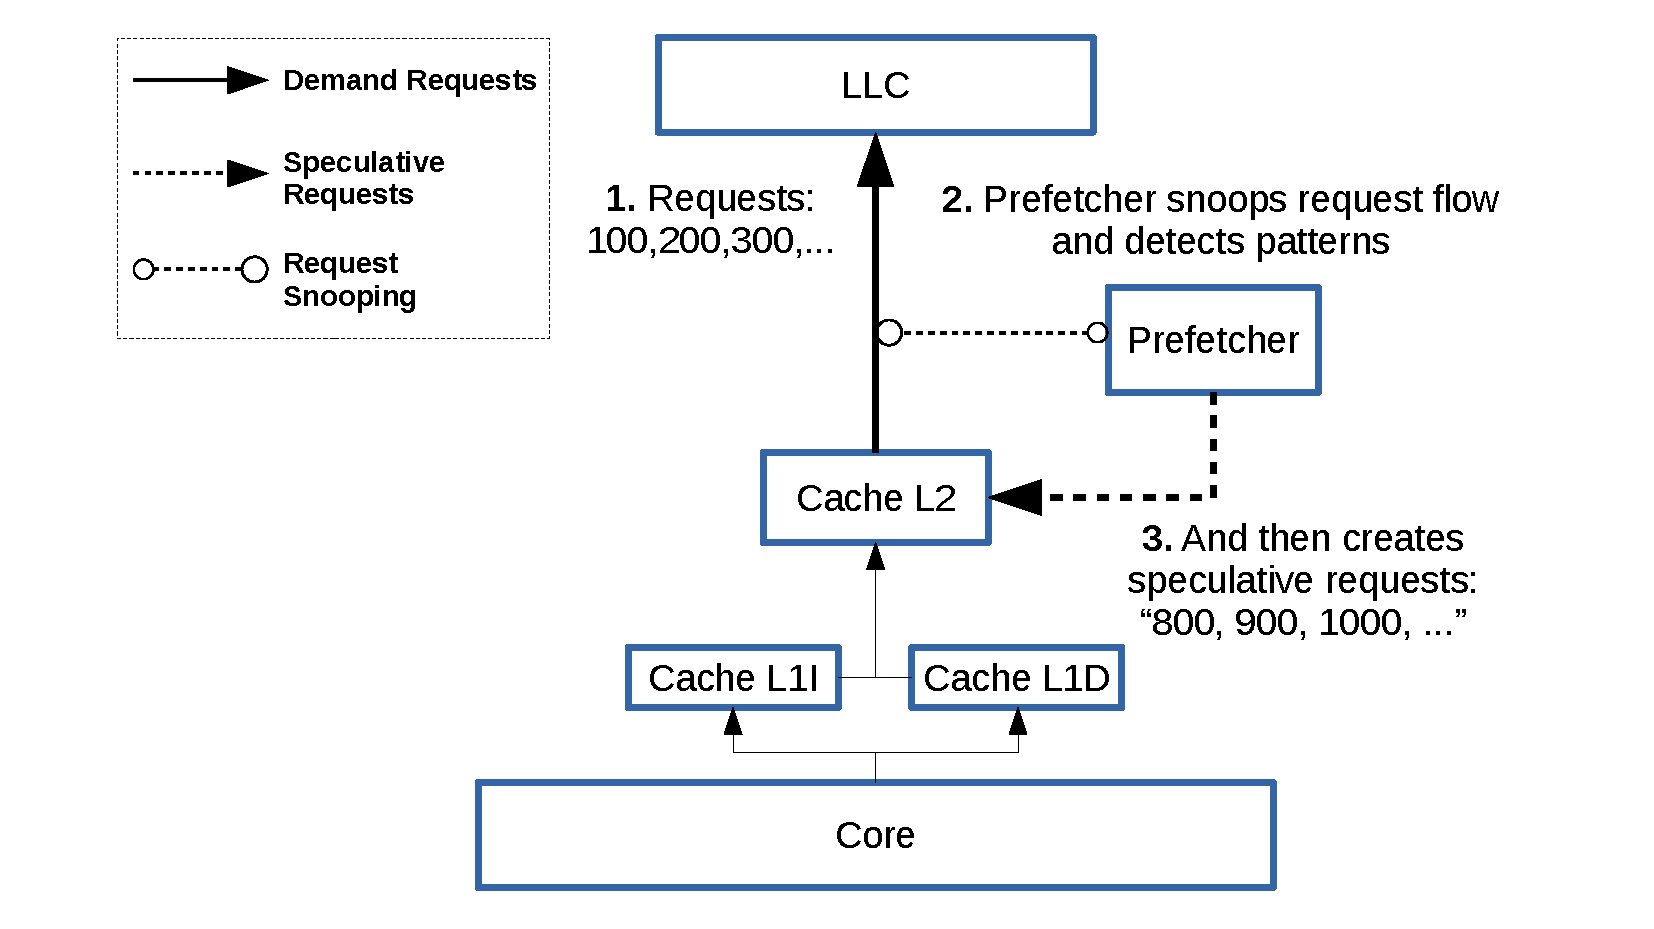
\includegraphics[width=.7\textwidth]{figures/figpref-en.pdf}
  \caption{Abstraction of the prefetcher behavior.}
  \label{fig:prefetcher}
\end{figure*}

Figure \ref{fig:prefetcher} shows an example of a second level of cache (L2) prefetcher detecting a stride access pattern.
The L2 cache forwards requests to the LLC (shown in Figure \ref{fig:prefetcher} as the event \textbf{1}).
The prefetcher, in turn, intercepts these requests by snooping the cache interconnection (\textbf{2}) and identifies the access pattern being generated.
Based on the pattern identified, speculative accesses are inserted into the L2 Miss Status Holding Register (MSHR) (\textbf{3}), a buffer that keeps track of miss events that still need to be handled.
These speculative requests are made directly to the L2 cache in order to avoid a redundant cache fill if the speculated line already resides in the cache.
These accesses are seen as regular requests made to the L2 by the prefetcher, so the L2 does not actually need to forward the response to the L1.
If the speculated address is not present in the L2 yet, the next levels in the hierarchy will forward the response to whoever requested it, as in a regular access.
Thus, when the processor needs the data requested by prefetch, it will already be at a closer cache level (in this case, the L2 cache).

\subsection{Simulators}

In computer architecture research, physical implementation and analysis are infeasible due to the complexity and high cost for manufacture. 
Consequently, architecture simulators are considered the primary mechanism to implement and evaluate a new ideas in this research field.
In High-Performance Computing (HPC) systems, there are many other problems besides those inherent to the architecture.
To develop and analyze new ideas that attenuate problems arising from parallelism, we require multicore architecture simulators that support parallel workloads.
For example, in systems with dozens of cores, problems such as the interference among the different threads and the communication costs among them must be modeled to obtain accurate results.
Thread interactions occur mainly through shared memory, with several threads accessing the same memory addresses, making necessary to keep data coherence in the several cache levels.
Thereby, parallel simulators must provide an accurate implementation of cache coherence protocols and ensure data consistency through the memory hierarchy.

In the following subsections, we present the two simulators used in this work, ZSim\cite{sanchez2013zsim} and Sniper\cite{carlson2014aeohmcm}.

\subsubsection{ZSim}\label{ref:subs_zsim}

ZSim was selected for our study due to its speed and accuracy, characteristics presented in its validation study~\cite{ZSim2016validation}.
It is an instruction-driven simulator that uses dynamic binary translation (DBT) to perform the instruction execution and dynamic instrumentation.
The simulation uses a two-phase method called Bound and Weave.
In the Bound phase, a few thousand cycles are simulated, ignoring the contention and applying a minimal latency for all memory accesses.
In this phase, a trace of all memory accesses is recorded, including which caches lines were accessed, evicted, invalidated, and so on.
In the Weave phase, a parallel simulation is performed, oriented to the events of the recorded interval to determine the actual latency of each memory request in each component.
Once the interactions between memory accesses have already been identified in the first phase, this timing simulation of these accesses can be done efficiently, maintaining high precision.

The authors observed that, in an interval of a few thousand cycles, most of the concurrent accesses between different cores happen to unrelated cache lines.
Therefore, simulating these unrelated accesses first out of order and ignoring contention and, later, simulating them in order respecting time constraints, is equivalent to simulating them entirely in order.
However, when accesses are related, i.e., access the same cache line, it is necessary to maintain the coherence of the different copies of the data in the different cores.
An example of this is when a core demands exclusive access over a shared cache line to write into it, causing the cache coherence protocol to invalidate the other copies of the line in the cache hierarchy system.

The set of requests and messages necessary to invalidate the other copies of the line to obtain it as exclusive is known as Request for Ownership - RFO.
However, for being considered rare, the order of these accesses to the same line is not modeled by ZSim, which can change the path of this data in the cache hierarchy.
Changing the path of the data through the cache can impact the number of cycles, misses, and coherence messages observed in the simulation.
In addition, the generation and the paths of prefetch requests can also change, preventing the modeling of prefetcher in this simulation model.

In its validation, ZSim uses the benchmark PARSEC \cite{bienia2008parsec} and only shows that the speed-up is close to that obtained with real executions by varying the number of threads.
Therefore, as the prefetcher is not simulated, we seek to understand the impact of its absence and evaluate the accuracy of the Bound and Weave method used to simulate multiple structures and threads in parallel. 

\subsubsection{Sniper}
\label{subsubsec:sniper}

Sniper is a simulator that extends the original interval simulation model~\cite{genbrugge2010interval} to improve its handling of overlapping memory accesses through a more detailed dependency analysis of memory accesses~\cite{carlson2014aeohmcm}.
The simulator presents the instruction-window centric (IW-centric) simulation model, a high-level core model that combines the interval modeling with a detailed simulation model of the instruction window, or reorder buffer (ROB)~\cite{carlson2014aeohmcm}.
The IW-centric simulation model focuses on accurately simulating the parallelism and latencies of instructions' execution in the processor. 
This is done by modeling micro-op dependency and issue timing in detail, estimating the performance by processing micro-ops out of order, in a way similar to how a real processor would issue them~\cite{carlson2014aeohmcm}.
However, the IW-centric model requires a longer simulation time.
For that reason, in this study we make use of their improved interval simulation model.

The basis for interval analysis is the observation that, in the absence of miss events such as branch mispredictions and cache misses, a well-balanced superscalar out-of-order processor should smoothly stream instructions through its pipelines, buffers, and functional units~\cite{eyerman2009model}. 
Under ideal conditions the processor sustains a level of performance (instructions per cycle) roughly equal to the superscalar dispatch bandwidth~\cite{eyerman2009model}. 
However, the smooth dispatch of instructions is intermittently disrupted by memory request miss events and branch mispredictions.
The effects of these events at the dispatch stage divide execution time into intervals, and these intervals serve as the fundamental entity for analysis and modeling\cite{eyerman2009model}.
The original interval modeling is itself a simulation model that allows the simulation of prefetchers in Sniper.

The interval simulation works with two structures named new window and old window.
Each window contains as many micro-ops as would exist in the reorder buffer (ROB) of an out-of-order processor~\cite{carlson2014aeohmcm}.
The new window represents the upcoming micro-ops and is fully filled the entire time, and the old window contains a list of the most recently dispatched micro-ops~\cite{carlson2014aeohmcm}.
The instantaneous IPC is calculated as the number of micro-ops in the entire old window divided by the latency of the micro-ops on the critical path~\cite{carlson2014aeohmcm}.
By repeating this process for each micro-op (and accumulating the leftover work for future micro-ops), Sniper can estimate the application’s instruction level parallelism (ILP) during the non penalty portion of an interval~\cite{carlson2014aeohmcm}.

In its validation, Sniper uses the benchmark SPLASH-2\cite{woo1995splash} and also shows that the average speed-up error is small when varying the number of threads.
Although Sniper provides an implementation of the prefetcher's behavior, it has only been recently validated for the Cortex-A53 and Cortex-A72 ARM cores~\cite{adileh2019racing}.
The prefetcher model is responsible for over half of the simulation error in the \emph{povray} and \emph{x264} benchmarks, as some implementation details of the real hardware are unknown.
However, the validation used only sequential benchmarks.
In contrast, this study contributes to a better understanding of the accuracy of the simulated prefetch model and how it behaves in simulations of parallel architectures.


\section{Related Work}\label{sec:related}

Due to the lack of explicit information that hardware companies employ to avoid competition and breaches of their intellectual property, it is difficult to obtain an accurate simulation that correctly presents all the characteristics of a processor and its architecture. 
Therefore, designers of a simulator seek a low relative error when validating their simulator, and tailor the details of the simulator to make it sensitive specifically to the desired area of design, e.g., memory hierarchy~\cite{eeckhout2010computer}. 

For instance, if we variate the amount of cache memory and try to simulate a target program that requires a large amount of cache memory, the simulator should indicate loss or gain of performance. 
If it does not, either it does not model the cache correctly or suffers from bottlenecks in other parts of the model.

\subsection{Improving Simulator Accuracy}

Microbenchmarks can be used to decrease error in basic architecture structures and as a form of reverse engineering of architectural features~\cite{fog2012microarchitecture}.
In Desikan et al.'s work~\cite{desikan2001measuring}, the authors faced the difficulty of obtaining accurate information and studied the relevance of this information when validating the SimpleScalar simulator~\cite{austin2002simplescalar}. 
By obtaining more information about the Alpha 21264 processor model in direct contact with the manufacturers, the authors were able to reduce the experimental microbenchmarks error from 19.5\% to 2\%.  
With the SPEC-CPU 2000 workload, the average experimental error went from 36.7\% to 18.2\%. 
The authors then showed how the resources found generate bottlenecks in different parts of the system than previously modeled in several articles, invalidating ideas that presented performance gains due to bottlenecks that did not exist.

A more recent work by Walker et al.~\cite{walker2018hardware} in this direction automates the process of finding the source of simulator error.
The main objective of the work is to obtain more accurate energy consumption models for gem5, but to do so they required a more accurate processor model. 
Using gem5 and the processor configurations provided by Gutierrez et al.'s gem5 validation~\cite{gutierrez2014sources}, Walker et al. created GemStone, a framework to find the sources of simulation error based on empirical hardware performance monitor counters (PMCs) models.
GemStone selects the events in gem5, correlating them with the PMC events, and at last, performs one regression analysis to approximate the relationship between hardware PMCs and gem5 error, and another to approximate the relationship between gem5 events and gem5 error.

\subsection{Prefetcher Simulation}

The development of new prefetching techniques is an active area.
Mittal~\cite{mittal2016survey} provides a survey on recent development of prefetching techniques up to 2016.
In the survey, the authors describe the relevant prefetch metrics, such as accuracy, coverage, and timeliness~\cite{srinath2007feedback}, as well as the different types of technique to improve prefetching, such as new pattern detection techniques~\cite{nesbit2004data}, filtering prefetches~\cite{zhuang2006reducing}, dropping prefetches~\cite{lee2008prefetcher}, changing prefetches' priority on the memory controller~\cite{ebrahimi2009coordinated}, and so on.
Given the variety of techniques and the active development of new techniques, one can hardly keep up with the design of prefetchers and additional techniques in the industry, which are not publicly disclosed.
Thus, most simulator designers face difficulties when modeling prefetchers, as they cannot real hardware information.
Interestingly, many of these techniques are not tested in multithreaded applications, where communication plays a major role in the memory hierarchy latency~\cite{jain2018rethinking,wu2019efficient,bhatia2019perceptron}, which we explore in this work.

\subsection{Simulator Survey} 

Since Desikan's work, several simulators have been created along a validation effort to evaluate their accuracy.
In Akram et al's research~\cite{akram2019survey}, the authors evaluated and compared the gem5~\cite{binkert2011gem5}, Multi2Sim~\cite{ubal2012multi2sim}, MARSSx86~\cite{patel2011marss}, PTLsim~\cite{yourst2007ptlsim}, Sniper~\cite{carlson2014aeohmcm}, and ZSim~\cite{sanchez2013zsim} simulators. 
After thorough characterization of the simulators, the authors tested single core and multiprogrammed workloads on each simulator. 
The results of each simulator were compared with the Intel's Haswell architecture~\cite{hammarlund2014haswell}. 
The authors then highlighted the error sources of the simulators, their sensitivity to different architectural parameters, and their relative error. 
Thus, they concluded that the lack of validation of a simulator for the target architecture, no matter how popular it is (e.g., gem5, which was only validated for ARM~\cite{gutierrez2014sources}), leads to low accuracy and may render experiments invalid due to erroneous conclusions.

However, Akram's work does not use multi-thread applications to verify the error relative to the number of threads and the accuracy of communication in these simulators.
The two best simulators in Akram's results, in terms of accuracy, were Zsim and Sniper, which we selected for this work.

\section{Methodology and Experimental Environment}\label{sec:experiments}
In this Section, we present details about the experimental environment and the prefetcher algorithms provided by the real machine hardware and by Sniper.
Moreover, we describe the methodology applied in the experiments, the benchmark used and the different prefetcher combinations executed and simulated.

\subsection{Experimental Setup}
\label{subsec:exp-setup}

\begin{table}[b]
    \centering
    \footnotesize
    \caption{Real machine, ZSim and Sniper configurations.}
    \label{tablehb}
    \renewcommand{\tabcolsep}{1pt}

   \resizebox{.8\linewidth}{!}{
    \begin{tabular}{{@{\hspace{0.0cm}} l @{\hspace{0.1cm}} @{\hspace{0.1cm}} c @{\hspace{0.1cm}} @{\hspace{0.1cm}} c @{\hspace{0.1cm}} @{\hspace{0.1cm}} c
    @{\hspace{0.1cm}} @{\hspace{0.1cm}} c @{\hspace{0.1cm}} @{\hspace{0.1cm}}}}
    \toprule
    & \bfseries Real &\bfseries ZSim  &\bfseries Sniper \\
    \midrule
    Processor Frequency & 2.1 Ghz & 2.1 Ghz  & 2.1 Ghz \\ 

    Number of Cores & 12 & 12  &  12 \\

    Pipeline Stages & 18 & 16  &  16\\

    \midrule
    Cache Line Size & 64~B & 64~B  & 64~B\\
    
	L1 Data Cache & 8-way 32~KB & 8-way 32~KB  & 8-way 32~KB\\
	
	Latency & 4 & 4  & 4\\
    \midrule
    
    L1 Instruction Cache & 8-way 32~KB & 8-way 32~KB  & 8-way 32~KB\\
	
	Latency & 4 & 4  & 4 \\
    \midrule
    
	Unified L2 Cache & 16-way 1~MB & 16-way 1~MB  & 16-way 1~MB\\
    
    Latency & ca. 14 & 14 & 14\\
    \midrule
    
    Last Level Cache L3 & Non-inclusive 11-way 16.5 MB & Inclusive 11-way 16.5~MB  & Inclusive 11-way 16.5 MB\\
    
    Latency & ca. 60-80 & 77 & 77\\
    \midrule
    Prefetchers & L1 IP Stride &  & Simple (Stride L1 Prefetcher)\\
                & Adjacent Line prefetcher & No Prefetcher & Global History Buffer  \\
                & L2 DCU Stream prefetcher & & (L2 Prefetcher)  \\
    \bottomrule
    \end{tabular}
    }
\end{table}

\new{To collect information about the application execution in the real machine, we make use of the PAPI~\cite{terpstra2010papi} tool.
PAPI allows the obtaining of hardware counters values, a set of registers that provide information about CPU events such as the number of instructions and the number of cycles.
In each real execution, only one hardware counter is evaluated, thus avoiding aggregations or approximations that the tool performs when calculating several metrics in the same execution.}
The performance and the real executions statistics were evaluated with 10 executions of each metric, for each benchmark.
The execution environment was composed of an Intel Xeon Silver 4116 CPU \textbf{with 2.1 GHz of frequency}, the Skylake microarchitecture~\cite{doweck2017skylake}.
The simulation environment is an approximation of the real hardware, respecting the simulators' limitations.
Each simulation was executed only once, and all statistics were extracted from the same simulation.
\textbf{All the executions in the real machine were performed with the Intel Turbo Boost~\cite{rotem2012turbo} technology disabled.}

\textbf{An important observation regarding Skylake's architecture is the change from an inclusive L3 cache to a non-inclusive one.
Skylake's predecessor architecture was Intel Broadwell, which applies an inclusive L3 cache, meaning that all data brought into the L2 cache is also brought into the LLC.
However, in non-inclusive L3 caches like the one used by Skylake, the data found at the L2 cache may or may not be found in the LLC, and there is no guarantee regarding how it will behave.
Which data is brought to which level depends on the application's access pattern, code and data sizes and their layout in the memory, and also on the inter-thread communication and sharing behavior.
}

Table~\ref{tablehb}  presents the configuration of the real machine and the processor simulated by ZSim and Sniper. 
The Sniper's out of order core model was based on the Nehalem architecture~\cite{carlson2011sniper}, while ZSim based its out of order core model implementation on the Westmere architecture~\cite{sanchez2013zsim}, a process shrink of Nehalem.
Therefore, both simulators present a 16 stages pipeline, while the real machine architecture may present between 14 and 19 stages~\cite{fog2012microarchitecture}.
Other parameters such as cache associativity and cache access latency are easy to configure in the simulators and can be found in~\cite{fog2012microarchitecture,doweck2017skylake}.

In Table~\ref{prefetches}, we present the description of the prefetcher algorithms considered in this work. 
The algorithms found in the L1 cache hardware are the Data Cache Unit (DCU) Prefetcher~\cite{intelmanual} and the DCU IP Prefetcher~\cite{intelmanual}.
The DCU Prefetcher, also known as the streaming prefetcher, is triggered by an ascending access to very recently loaded data. 
The processor assumes that this access is part of a streaming algorithm and automatically fetches the next line.
The DCU IP Prefetcher keeps track of individual load instructions (based on their instruction pointer's value). 
If a load instruction is detected to have a regular stride, then a prefetch is sent to the next address which is the sum of the current address and the stride.

The L2 Hardware Prefetcher~\cite{intelmanual} and the L2 Adjacent Cache Prefetcher~\cite{intelmanual} are the prefetcher algorithms found in the real machine L2 cache.
The L2 Hardware Prefetcher monitors read requests from the L1 cache for ascending and descending sequences of addresses. 
Monitored read requests include L1 data cache requests initiated by load and store operations and also by the L1 prefetchers, and L1 instruction cache requests for code fetch.
When a forward or backward stream of requests is detected, the anticipated cache lines are prefetched.
This prefetcher may issue two prefetch requests on every L2 lookup and run up to 20 lines ahead of the load request. 
The L2 Adjacent Cache Prefetcher fetches two 64-byte cache lines into a 128-byte sector instead of only one, regardless of whether the additional cache line has been requested or not.

The prefetcher algorithms in Sniper are the Simple and the Global History Buffer (GHB)~\cite{nesbit2004data}.
Based on an analysis of the Simple prefetcher's code, we observed that it is similar to a strided prefetcher algorithm.
Thus, we use the Simple prefetcher as the L1 cache prefetcher in our experiments.
The GHB prefetcher is an $n$-entry FIFO table that holds the $n$ most recent L2 misses addresses. 
Each GHB entry stores a global miss address and a link pointer that is used to chain the GHB entries into address lists. 
Each address list is a time-ordered sequence of addresses issued by the same instruction pointer.
Therefore, based on the information of the address lists, it is possible to implement a correlation based prefetcher~\cite{charney1995GeneralizedCB} and a stride prefetcher~\cite{nesbit2004data}.
The L2 prefetcher found in Sniper is a GHB correlation based prefetcher, and in our experiments it is used as the L2 cache prefetcher.


Therefore, based on the aforementioned prefetchers, we conducted experiments on the real machine considering: %\textcolor{red}{\textbf{ATUALIZAR AQUI QUANDO OS GRÁFICOS NOVOS EM R ESTIVEREM PRONTOS!!!!}}
\begin{itemize}
    \item All Skylake's L1 cache prefetchers, henceforth "Real-L1 prefetcher", or simply L1 prefetcher;
    \item All Skylake's L2 cache prefetchers, henceforth "Real-L2 prefetcher", or simply L2 prefetcher;
    \item All Skylake's prefetchers from both L1 and L2 cache, henceforth "Real-L1-L2 prefetcher", or simply L1+L2 prefetcher;
    \item No prefetcher, henceforth referred to as Real-No Prefetcher.
\end{itemize}

Based on the Sniper's prefetchers, the following systems were simulated:
\begin{itemize}
    \item Only the L2 data prefetcher (GHB), henceforth "Sniper-L2 prefetcher", or simply Sniper's L2 prefetcher;
    \item Both L1 (Simple) and L2 (GHB) prefetchers, henceforth "Sniper-L1-L2 prefetcher", or simply Sniper's L1+L2 prefetcher;
    \item No prefetcher, henceforth referred to as Sniper-No Prefetcher.
\end{itemize}

Since ZSim does not model the prefetcher behavior, there are no variations of the simulated system. With ZSim we only perform simulations with no prefetcher, which we refer to as ZSim.


\begin{table}[]
    \centering
    \footnotesize
    \caption{Prefetcher algorithms.}
    \label{prefetches}
\resizebox{1.0\linewidth}{!}{
\begin{tabular}{@{}c|c|c|c|c|c@{}}
\toprule
\textbf{}                 & \textbf{Description}                                                           & \textbf{L1} & \textbf{L2} & \textbf{Real} &  \textbf{Sniper  } \\ \midrule
DCU Prefetcher   & 
Streaming prefetcher, fetches the next cache line into L1-D Cache  & \checkmark 
&   & \checkmark  &       \\
DCU IP Prefetcher         & 
Strided prefetcher of next L1-D line based upon sequential load history & \checkmark & & \checkmark  &       \\
L2 Hardware Prefetcher       & Mid Level Cache (L2) streamer prefetcher                                       &             & \checkmark  & \checkmark  &                \\
   L2 Adjacent Cache Prefetcher & Prefetching of adjacent cache lines into L2 Cache                                          &             & \checkmark & \checkmark  &                  \\
Simple & Strided prefetcher of L1-D line & \checkmark &  & & \checkmark \\ 
Global History Buffer & L2 Prefetcher based on global miss addresses & & \checkmark & & \checkmark \\
\end{tabular}
}
\end{table}

 

\subsection{NAS Parallel Benchmarks}
\label{subsec:nas}


For this study, we used a known HPC benchmark in the literature called Numerical Aerodynamic Simulation Parallel Benchmark (NPB)~\cite{jin1999openmp}. 
\new{This set of applications comprises ten applications, each of which encapsulates a certain type of computation that is often processed by HPC applications, e.g. computational fluid dynamics (CFD), adaptive meshes, parallel I/O, and computational grids.
We used nine of the ten NPB applications, namely: CG (Conjugate Gradient), EP (Embarrassingly Parallel), FT (Fourier Transform), IS (Integer Sort), MG (Multi-Grid), UA (Unstructured Adaptive mesh), BT (Block Tri-diagonal solver), LU (Lower-Upper Gauss-Seidel solver), and SP (Scalar Penta-diagonal solver).
The Data Cube (DC) application was discarded because DC mainly stresses I/O operations, which are not modeled by the architecture simulators.}



\new{The benchmark set presents different input classes that offer different input sizes and complexities.
The available input classes are: S, W, A, B, C, D, E, and F.
The class S was designed for quick testing purposes; class W was originally designed for standard testing considering a 90's workstations, and nowadays is used for quick test purposes as well; classes A, B, and C are standard test problems, whose size increases four times from one class to another; and classes D, E, and F, for large-size problems, whose size increases sixteen times from one to another.}




\section{Investigating Current Architecture Prefetchers}\label{sec:real_ipc}

In this section, we present the main results obtained by the aforementioned experimental setup, taking into account the real execution of the NPB benchmark. 
More specifically, here we shed light to the following question: \new{\textit{How do the different prefetchers affect the execution of NPB over a real machine with a varying level of parallelism?}}



Figure~\ref{fig:ipc} shows the instructions per cycle (IPC) for each NPB application, using the input class A, taking into account different numbers of threads and prefetchers, and with hardware prefetcher disabled as well. 
The IPC can be understood as a general performance metric of the prefetchers when executing the applications, since an efficient prefetcher will enable more processed instructions per cycle \new{by fetching the right data at the right time}. 
The error bars represent the variability observed among both the cores of a certain execution and the 10 distinct repetitions of the executions.


\begin{figure}[b]
    \centering
    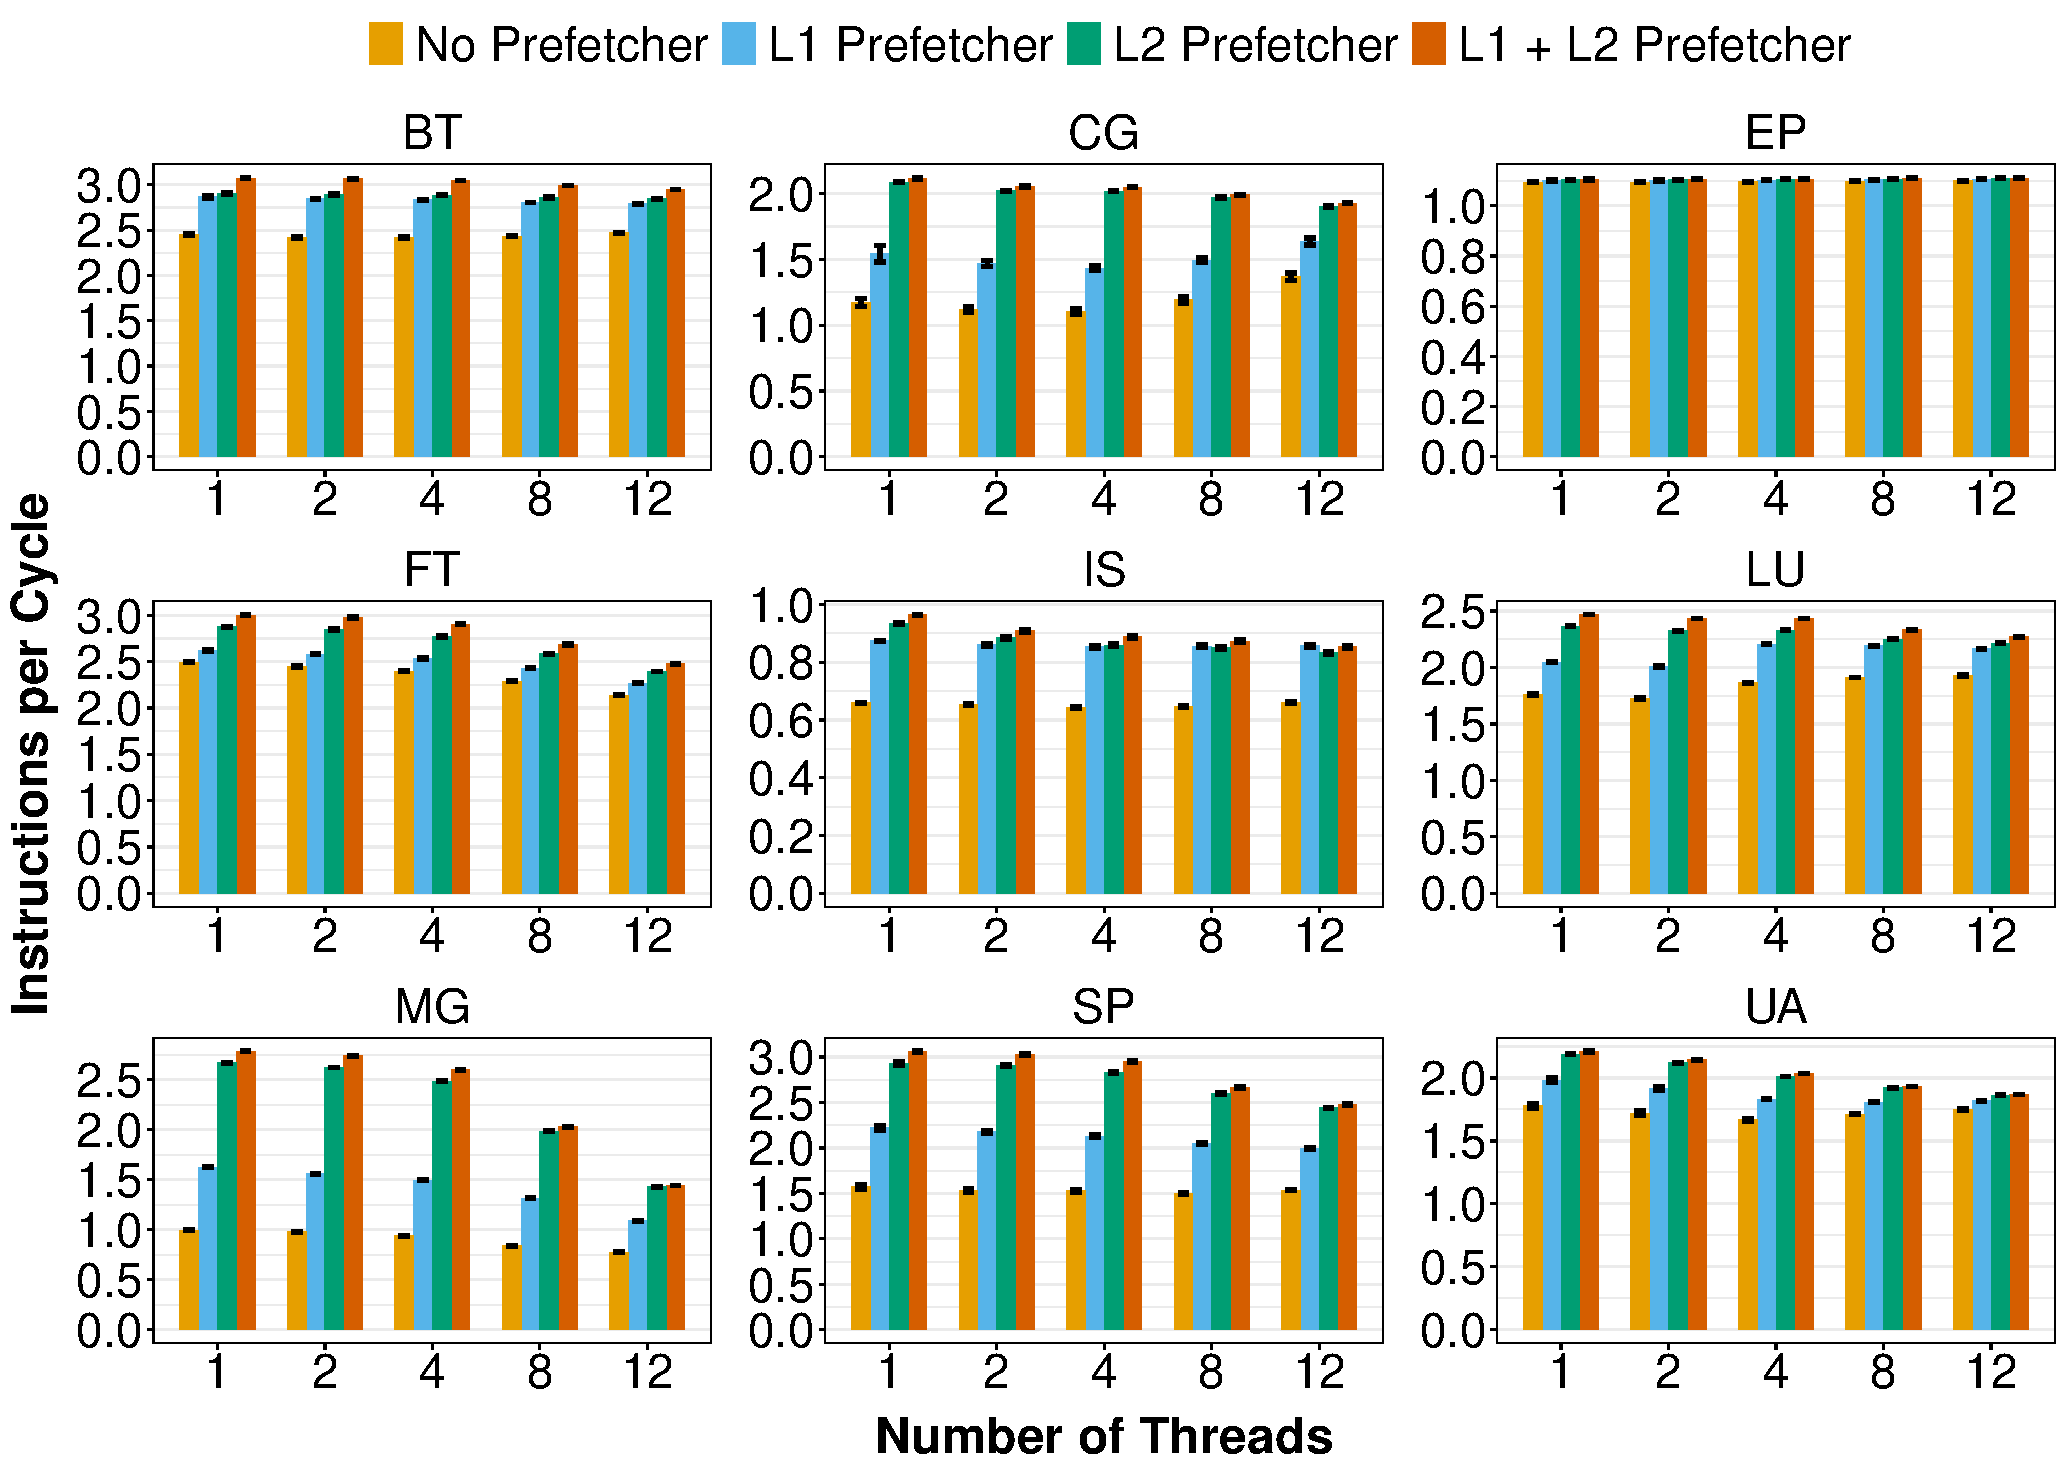
\includegraphics[width=\linewidth]{figures/fig2.pdf}
    \caption{IPC results for the real execution of the NPB applications with input class A.}
    \label{fig:ipc}
\end{figure}


As expected, we can observe that any prefetcher increases the execution performance of NPB, with the exception of the EP application. 
Since EP is known to have a small memory footprint~\cite{jin1999openmp}, processor stalls due to memory access latency rarely occur during its execution. 
Therefore, there is little difference in the IPC given different prefetcher configurations for EP. 
For the other applications, memory prefetching significantly contributes to a better IPC, specially for executions up to four threads.

\new{However, the increase in performance from a standalone L2 prefetcher to the combination of L1+L2 prefetchers is not as large, with an overall average IPC improvement of 2.9\%, when compared to the 31.9\% of performance increase from no prefetcher to the standalone L2 prefetcher.}
\new{This can be explained by the L2 prefetcher's ability to detect more relevant memory access streams that are dependent on the LLC's long-latency response, while the L1 prefetcher detects access to data that might be found at the on-core L2 cache level.}
Since the difference in latency from L1 to L2 is small, and the latency from L2 to LLC is much larger, this means the main performance gains would be obtained by the L2 prefetcher and the associated access streams it detects.
For concrete numbers, the L2 cache access latency is of 14 cycles, only 10 cycles higher than the L1 cache, while the LLC latency in Skylake is measured to be approximately between 60 and 80 processor cycles, presenting a much more substantial overhead and a higher probability of stalling the processor execution~\cite{alves2015sinuca}. 
\new{Furthermore, in Figure~\ref{fig:real_l2-rqsts-all-pf} we present the sum of all prefetch requests performed by the active prefetchers of each active core in the real execution, also for the input class A.
We can observe that, for some applications (e.g. BT, FT, SP, and some executions of LU), the number of prefetch requests performed by the L1 prefetcher is larger than the number of requests performed by the L2 prefetcher, and, in some cases, it almost reaches the same amount of requests performed by the two prefetchers combined (the L1+L2 executions).
Despite the L1 prefetcher issuing more prefetches than the L2 prefetcher in several cases, the fewer L2 prefetches are the ones who deliver the most crucial performance gains, as seen in Figure~\ref{fig:ipc}.}

\new{Another complementary explanation for this small performance gains observed for the L1 prefetcher is that its requests may be detrimental to performance, since they may compete with demand data for the rather limited cache space on the L1 cache level.
Moreover, these prefetch requests may also occupy too many entries on the line fill buffers present in the L1 hardware, competing again for shared and limited resources with the critical demand accesses, which are more relevant for the immediate processor execution than the prefetched lines.}


The \new{L1+L2} prefetcher combination is often set as the default setting in the machine configurations.
One of its main appeal is that it is the setting that provides the best performance. 
\new{However, one drawback of this approach lies in the interpretability of what is being performed by the algorithms.
The lack of understanding over the full prefetcher hierarchy behavior hinders the accurate implementation of prefetching models in architecture simulators, which will be demonstrated in detail in Section~\ref{sec:simulation}}.
For instance, the interactions between the prefetchers of each cache level (e.g., whether the L2 prefetcher considers L1 prefetches as part of the application's access stream or as prefetch requests) can cause major changes in the behavior of the memory hierarchy.
In contrast, the L2 prefetcher in isolation provides a simpler, more transparent understanding of the prefetches performed by the algorithm, facilitating reverse engineering and reproduction or simulation of the prefetcher, almost reaching the best observed performance (L1+L2).
At the light of these results, it may be advisable to set the L2 prefetcher on its own, as opposed to the L1+L2 setting, since the lack of transparency in the details of the L1 and L2 prefetcher, the L1 line fill buffer contention, and the additional energy consumption of the L1 prefetcher may not outweigh its increase in performance.



Another interesting trend observed in Figure~\ref{fig:ipc} is the decrease in the IPC for increasing number of threads in the majority of applications and prefetchers, with the exception EP application.
Apart from EP -- which, for the same reasons explained above, the IPC is stable for any number of threads on all cores -- the NPB applications use memory accesses and inter-thread communications, that naturally increase in function of the total number of threads. 
With a large number of threads, these memory accesses and inter-thread communications generate contention that become a larger constraint in the IPC, and the performance provided by prefetchers becomes small or negligible. 
\new{This effect can be clearly seen in the IPC graph for the MG application: MG is known to use memory-intensive operations and to be communication-intensive, largely benefiting from memory prefetchers. 
However, as the number of threads increases, the contention becomes a more considerable constraint in the IPC results, significantly harming the performance.}


In this regard, we hypothesize that, when the number of concurrent threads executed in a processor is high, the performance benefit from memory prefetchers for applications that use intense memory and inter-thread communications is negligible. 
\new{These characteristics would need to be alleviated on the applications for memory prefetchers to be effective.} 
However, an interesting exception to this observation is the CG application's executions with the L1 prefetcher and without prefetcher (Figure~\ref{fig:ipc}), where the IPC increases in function of the number of threads. 
We explain the CG case with more details in Section~\ref{subs:cg}.

\begin{figure}[!htb]
    \centering
    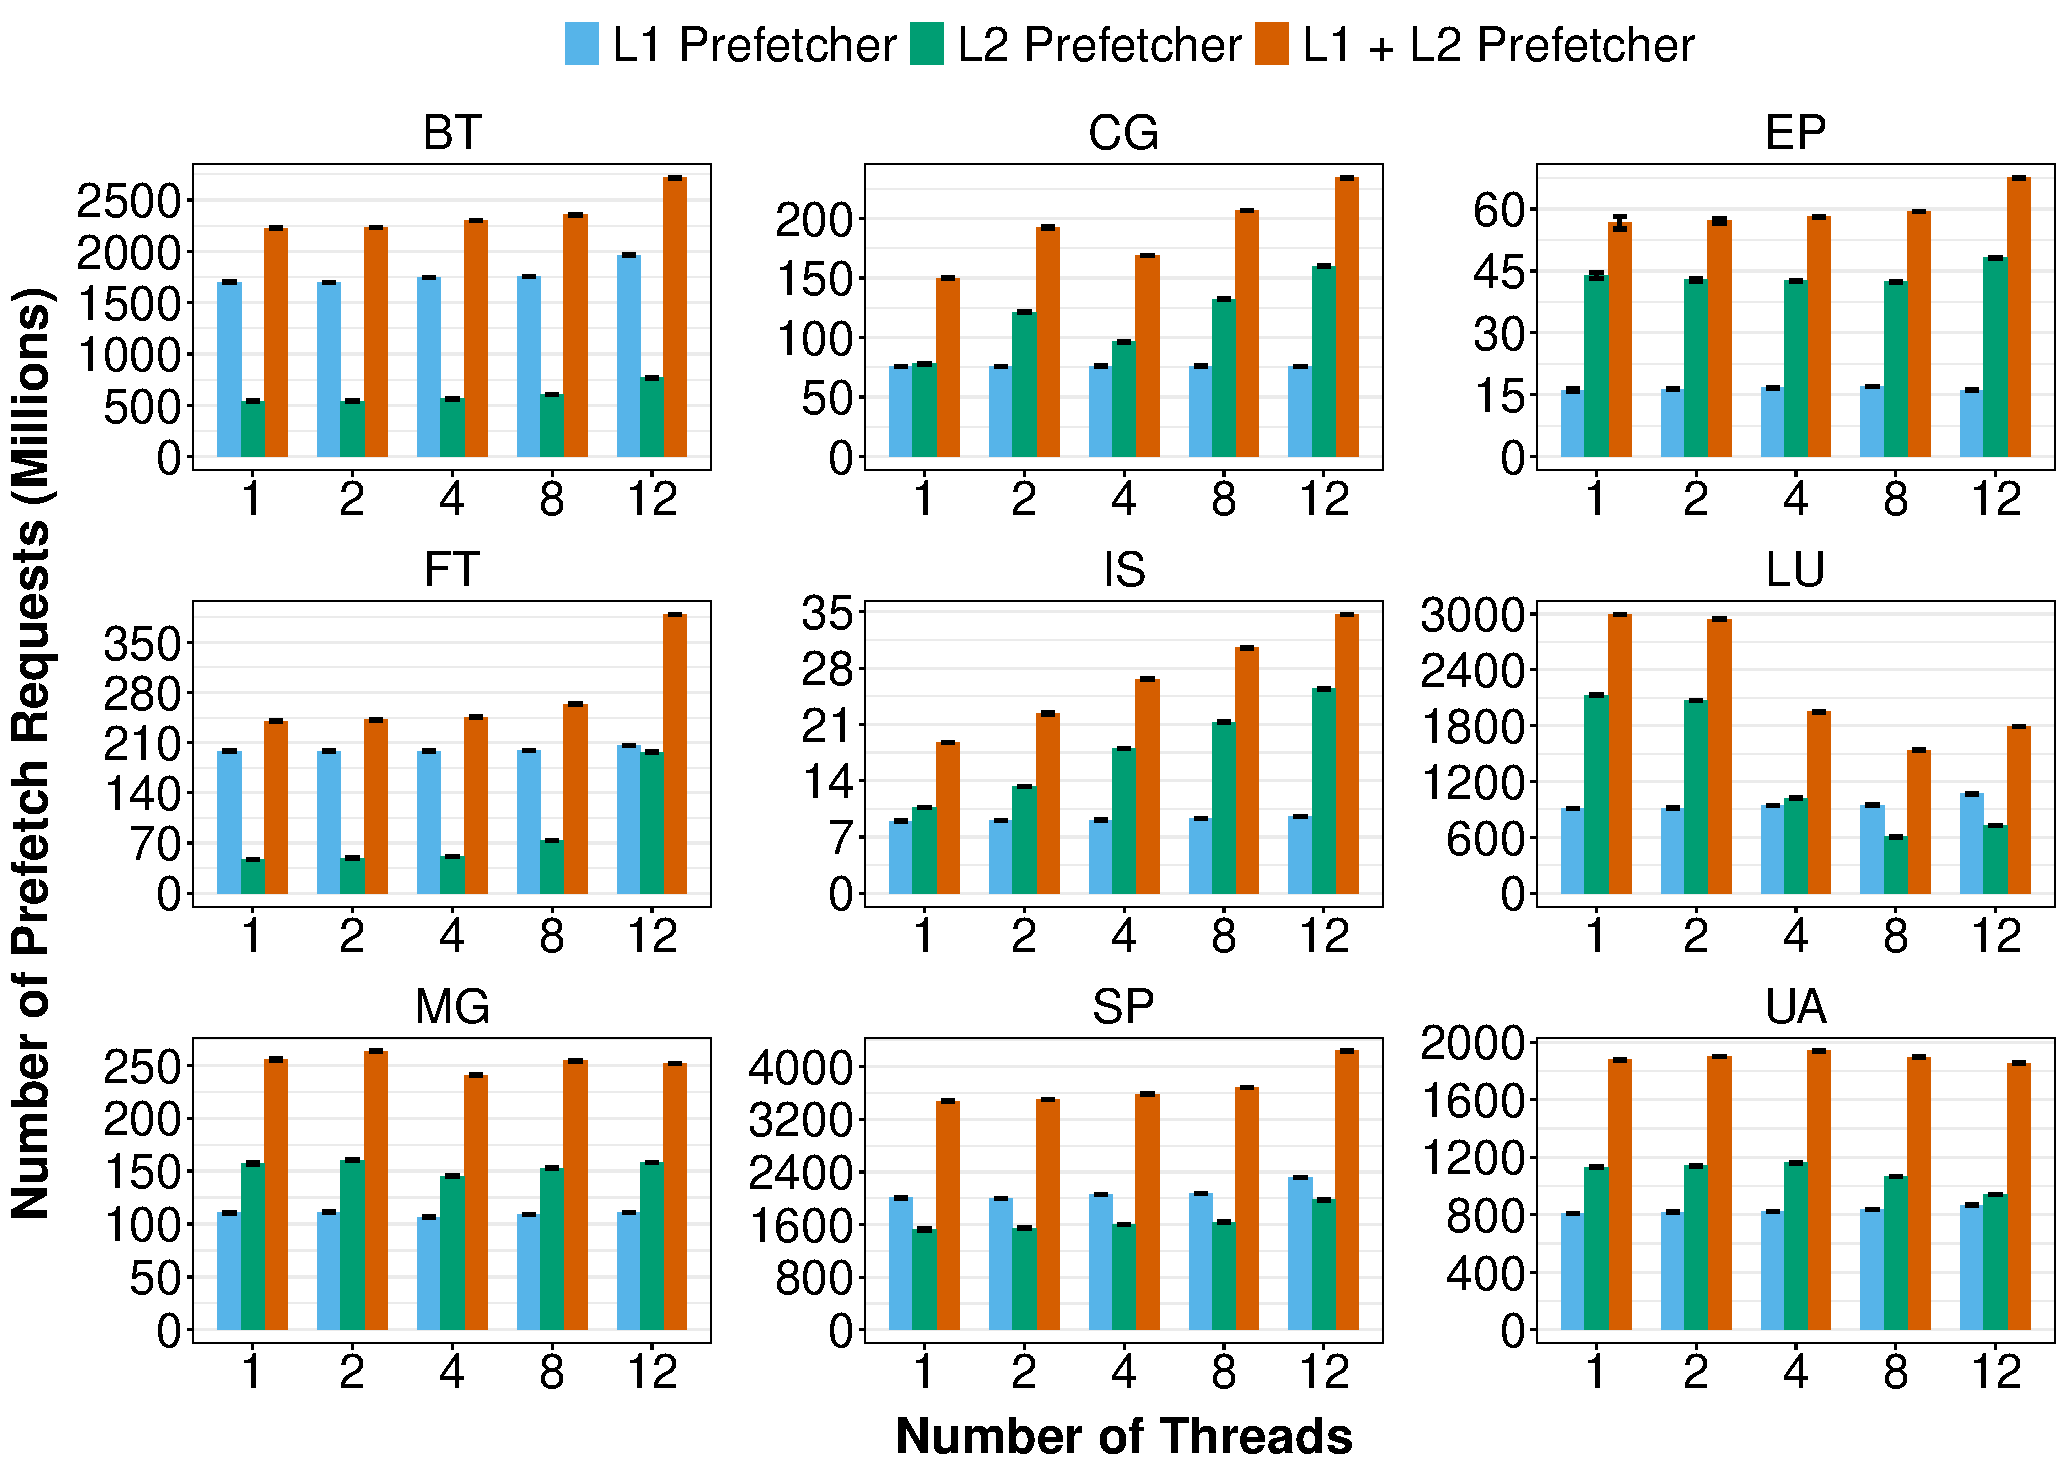
\includegraphics[width=\linewidth]{figures/fig3.pdf}
    \caption{Number of prefetch requests of the real machine executions with the input class A.}
    \label{fig:real_l2-rqsts-all-pf}
\end{figure}



\subsection{The CG Case}\label{subs:cg}


As previously explained, all NAS applications, except CG, suffer from a performance decrease as a result of the increasing memory contention that harms the prefetcher's efficiency in highly parallel applications.
However, the CG executions with the L1 prefetcher and without prefetcher present a contrasting behavior, with the IPC increasing in function of the number of threads, as demonstrated in Figure~\ref{fig:ipc}.
This section aims to detail the CG executions to better understand the CG results, showing how the application behavior contributes to the different observations. 


\begin{figure}[!htb]
    \centering
    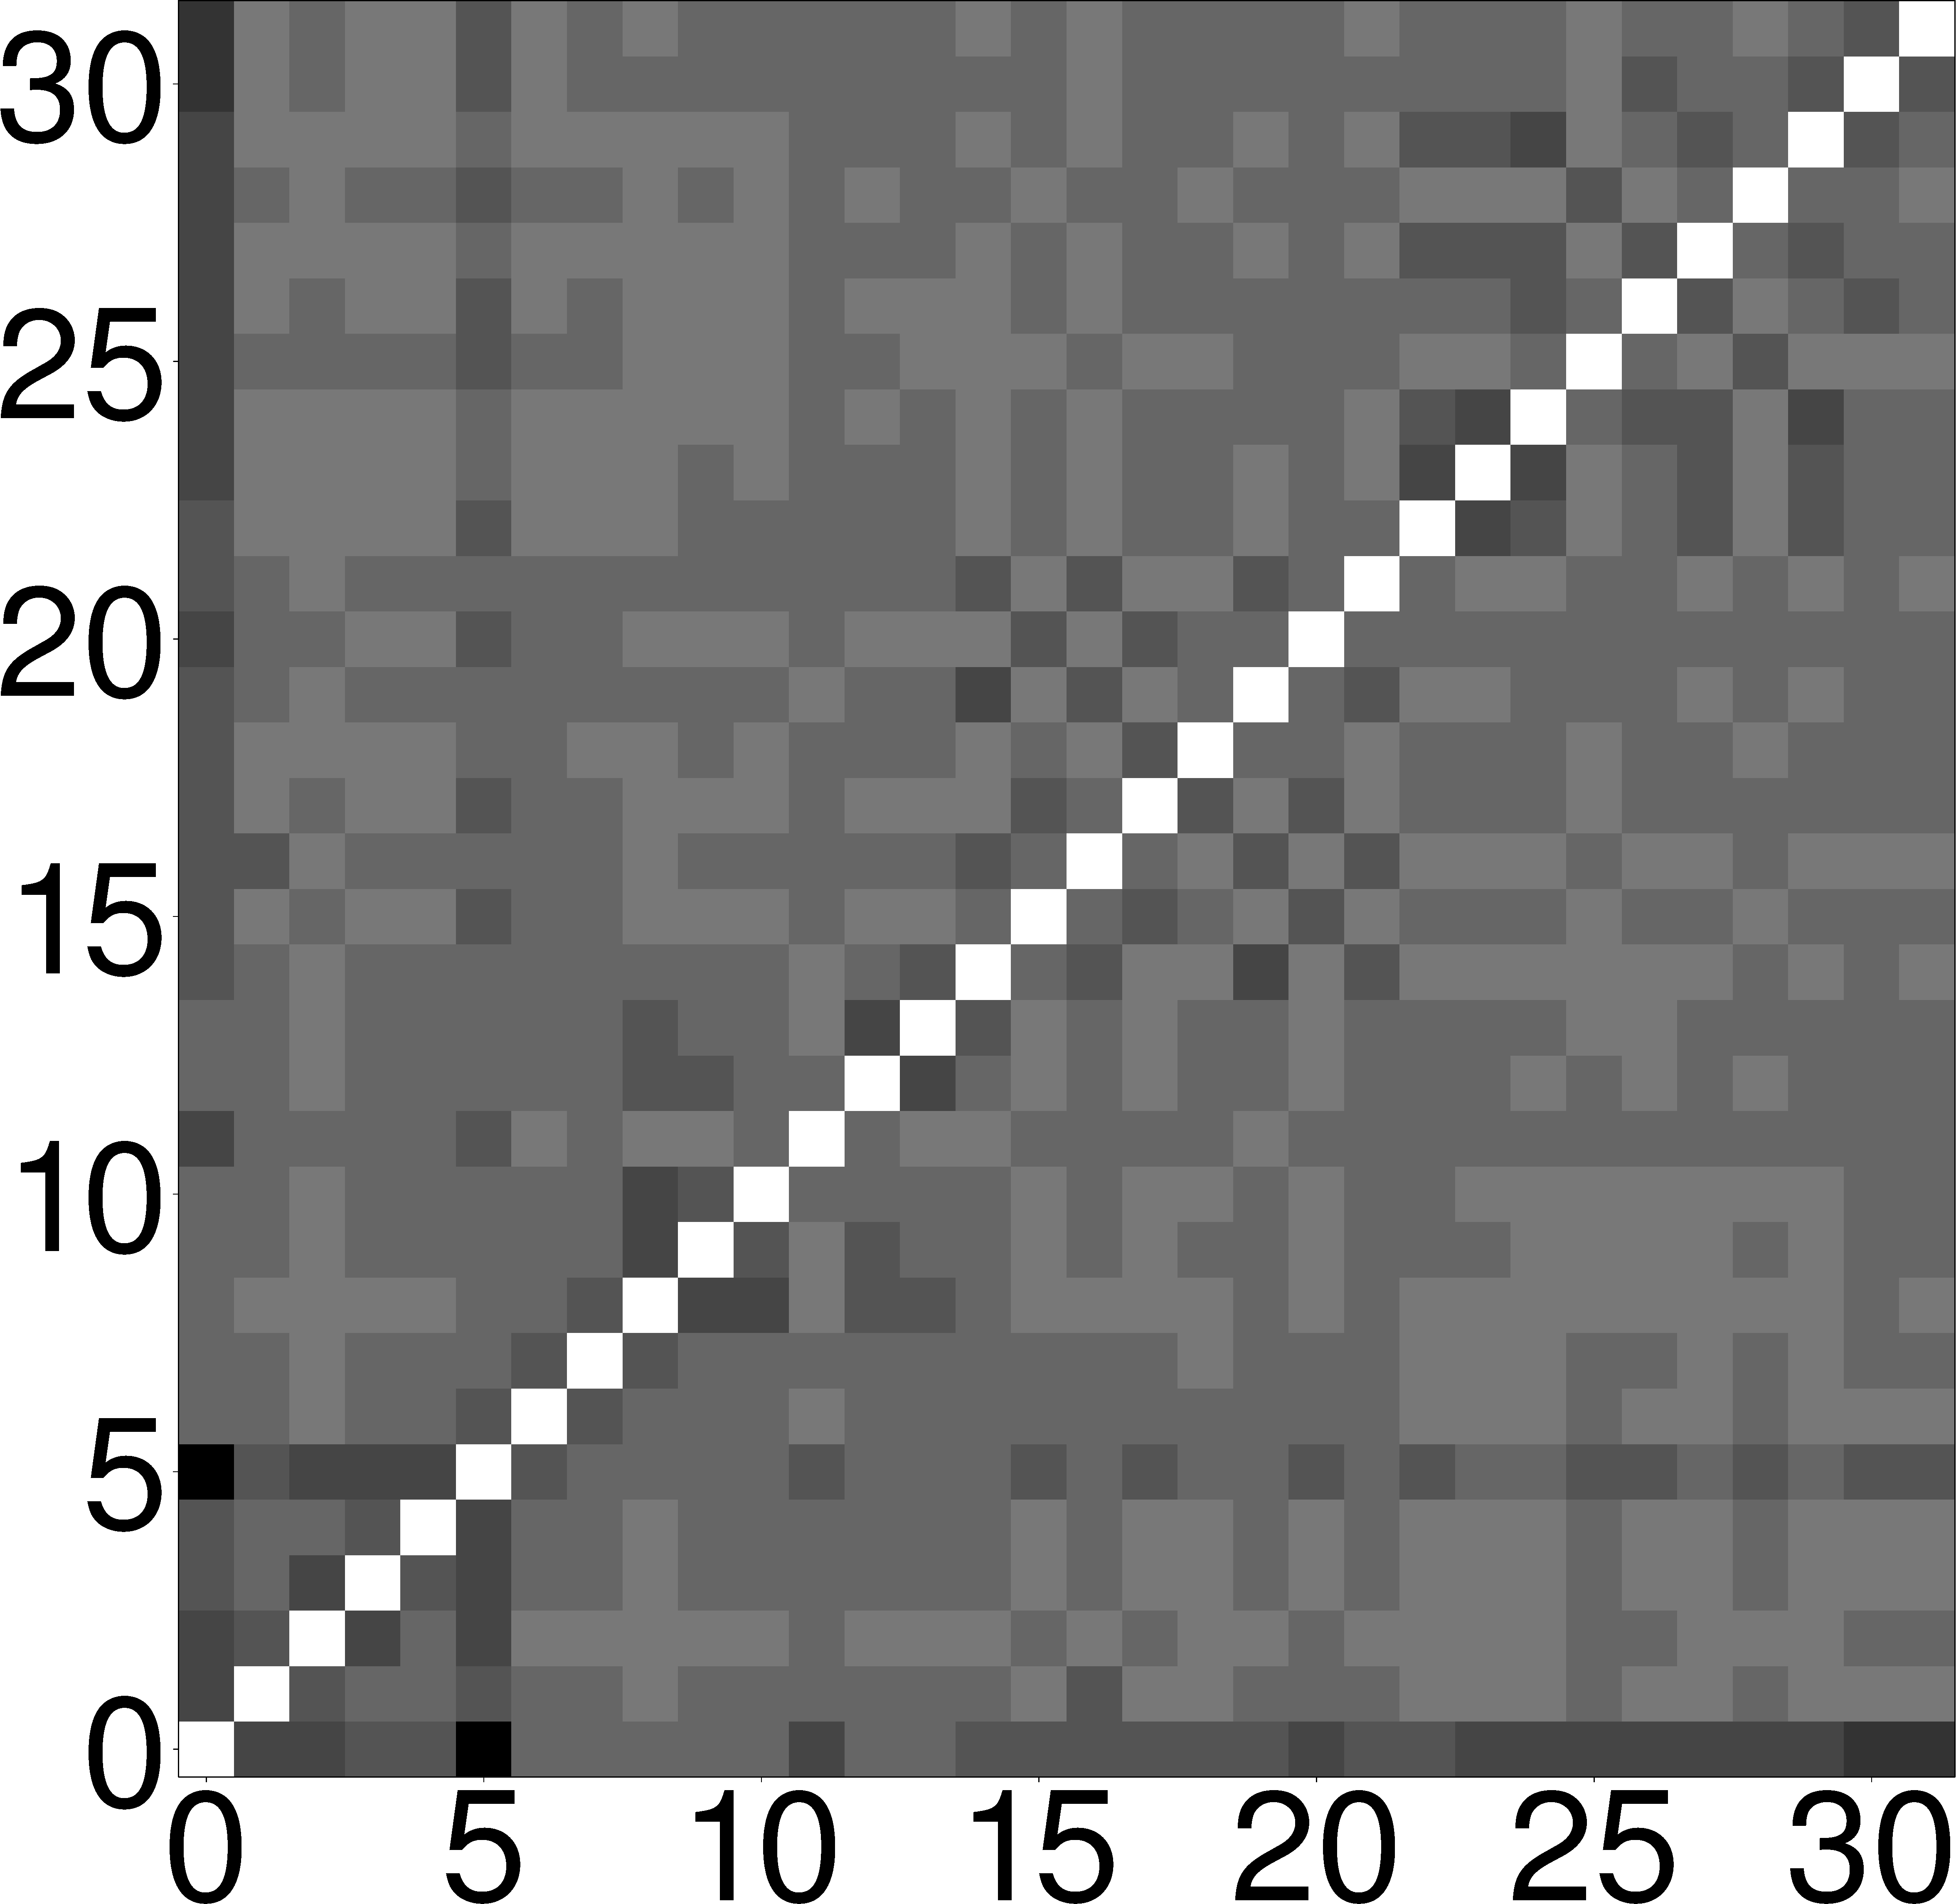
\includegraphics[width=.3\linewidth]{figures/cg.pdf}
    \caption{CG communication pattern for 32 threads. Figure obtained from: Cruz \textit{et al.}~\cite{cruz2018thread}}
    \label{fig:figcomma}
\end{figure}



First, we can observe CG's communication pattern in Figure~\ref{fig:figcomma}.
In this figure, the darker a given cell is, the more shared memory accesses occurred between the threads represented by row and column.
The diagonal is filled with white as a thread does not share data with itself.
Thus, we can see that all threads of CG irregularly communicate with all threads, as described in Section~\ref{subsec:nas}.
These irregularly distributed memory accesses enable one thread to request a memory address that had already been requested by another thread or even by another thread's prefetcher.
Since the chosen processor model has a non-inclusive L3 cache (as mentioned in Section~\ref{subsec:exp-setup}), the data found in the L2 cache is not necessarily duplicated at the L3 cache as would happen in an inclusive cache hierarchy, resulting in more available cache space.
Therefore, as we increase the number of threads, the amount of cache space available for the application is increased by using each core's private cache levels (which include an 1 MB L2 cache per core).
Consequently, a larger part of the working set of the application fits inside the processor caches, reducing the number of LLC misses, and thus reducing the number of long-latency DRAM accesses as well. 


This behavior is shown in Figure~\ref{fig:drampapi}, where we depict the number of DRAM accesses as we increase the number of threads.
The instruction prefetcher has not been disabled for any of these executions, which explains the presence of prefetch requests when the hardware data prefetchers are disabled.
As we use more threads, fewer DRAM accesses need to be performed regardless of the prefetching mechanism, precisely because the application has the necessary data present in the cache.
Moreover, a more prominent decrease is observed on the demand read DRAM accesses for the executions without prefetcher.
These avoided DRAM accesses play an essential role in the performance improvements observed in these executions.
A prefetcher is accurate if it can hide the main memory latency by effectively pulling data from the main memory to cache memory before a demand access requests the data.
An accurate prefetcher should also generate a number of prefetches similar to the number of demand requests generated by the processor without prefetchers, i.e., the actual number of load/write instructions that would require data.
Otherwise, it is generating unnecessary main memory accesses to bring data that will not be used.
This does not necessarily reduce the IPC, but it can increase main memory contention, energy consumption, and cache pollution.
Within this context, Figure~\ref{fig:drampapi} shows that the L1 prefetcher is quite inaccurate, generating many more speculative accesses to the DRAM in comparison with the execution without prefetcher. 
In stark contrast, the L2 prefetcher on its own is a lot more accurate, as the total number of DRAM accesses for each number of threads is close to the case of no prefetching. 

\begin{figure}[!htb]
    \centering
    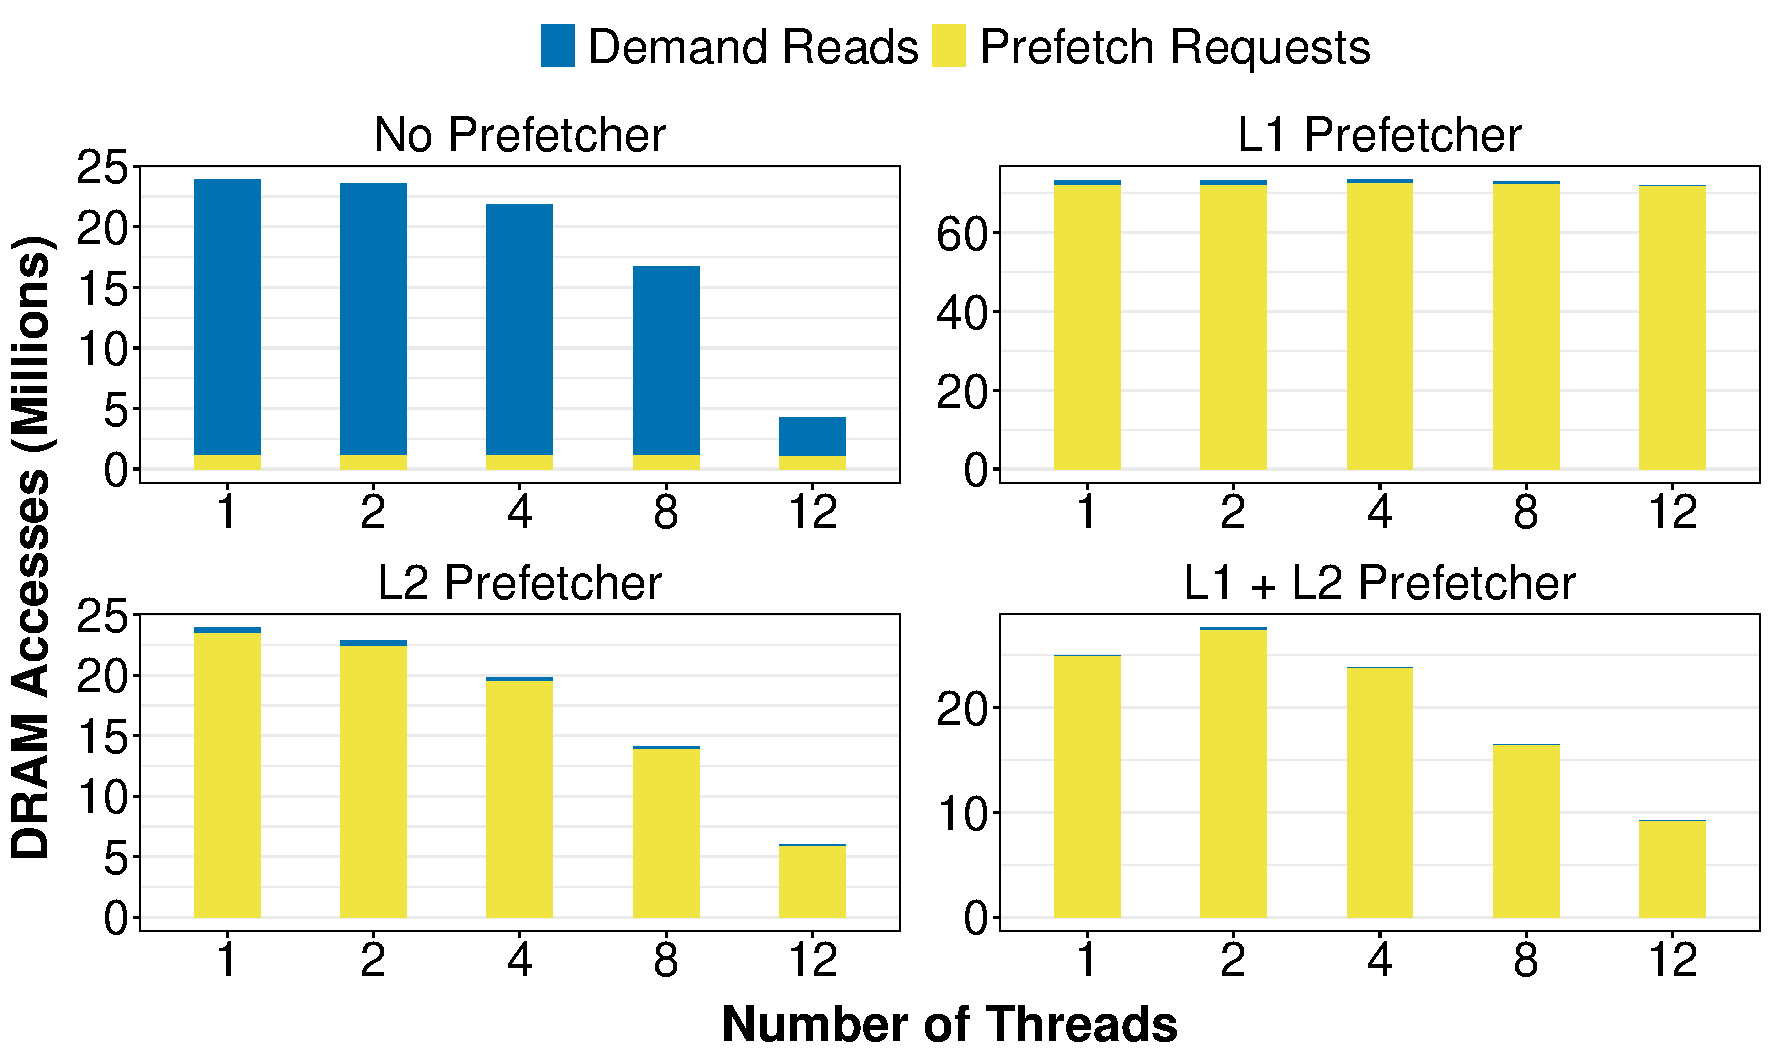
\includegraphics[width=.8\linewidth]{figures/fig4.pdf}
    \caption{CG main memory accesses, originated by demand reads and prefetches requests, for input class A.}
    \label{fig:drampapi}
\end{figure}


In Figure~\ref{fig:ipc}, we also notice a contrast in the performance of configurations with the L2 prefetcher, and those without.
Configurations with the L2 prefetcher do not have an IPC increase with a higher number of cores, as the L2 prefetcher is correctly speculating and bringing the data to the caches even with a low core count and low amount of cache.
On one hand, the IPC tendency of configurations with an L2 prefetcher is to decrease, as the prefetcher effectively hides the latency of DRAM accesses, but increasing the number of cores generates contention in the DRAM access.
On the other hand, configurations without the L2 prefetcher cannot hide this latency, and their IPC increase as the application is able to retain larger portions of the working set in higher quantities of private non-inclusive L2 caches.



\subsection{Effects of Different Input Classes}
\label{subs:NAS_WAB}


Up to this point, we analyze the relationship between the prefetcher and the parallelism increase with fixed input size.
However, the memory requirements of different HPC applications may vary substantially, requiring different execution parameters. 
For instance, when considering small input sizes, an execution with several threads may highlight communication effects, which will play a decisive role in the application's performance.
Simultaneously, the prefetcher's effectiveness may also be disturbed if we increase the parallelism in communication-intensive applications.
In this section, we aim to better understand how the prefetcher influences performance when we vary the application's memory requirements. 


In Figure~\ref{fig:nas_wab}, we present the IPC results for the SP application with different thread counts, different hardware prefetcher configurations, and variable input sizes, using NPB classes W, A, and B.
We present the results only for the SP application since the same behavior is observed for all other NPB applications.
The first point to be noted is that as we increase the problem size, the prefetcher's influence on the application's performance increases as well. 
If no prefetcher is enabled, class W suffers from a modest performance loss, while classes A and B are able to improve their performance by up to two times with all prefetchers activated.
Since class W has smaller memory requirements, any prefetcher that can predict a simple access pattern may already be able to fetch a significant part of the application's working set in advance.
Therefore, the performance decrease observed as we increase parallelism in class W is caused by the thread communication overhead observed over small input sizes, which can not be entirely solved by the prefetcher.

When we compare the performance reduction observed with the increase of parallelism for classes A and B, we identify that a bigger problem size suffers from a more dramatic loss.
As we increase the parallelism of the execution with the class A, the execution without prefetcher does not suffer performance reduction.
For class B, however, a small performance loss is observed even with all hardware prefetchers disabled.
This points out that the source of performance loss for class A is strictly related to the previously noted contention that arises with the prefetcher action in a multicore system.
For class A, the working set appears to fit entirely within the on-core memory levels; consequently, the application only demonstrates performance loss when facing prefetcher-related contention.
However, as the problem size scales, more off-core long-latency memory accesses are necessary since the working set does not fit entirely inside the on-core memory levels.
For this reason, these long-latency memory accesses, together with the prefetcher-related memory contention, harm the application's performance more fiercely in class B.


\begin{figure}
    \centering
    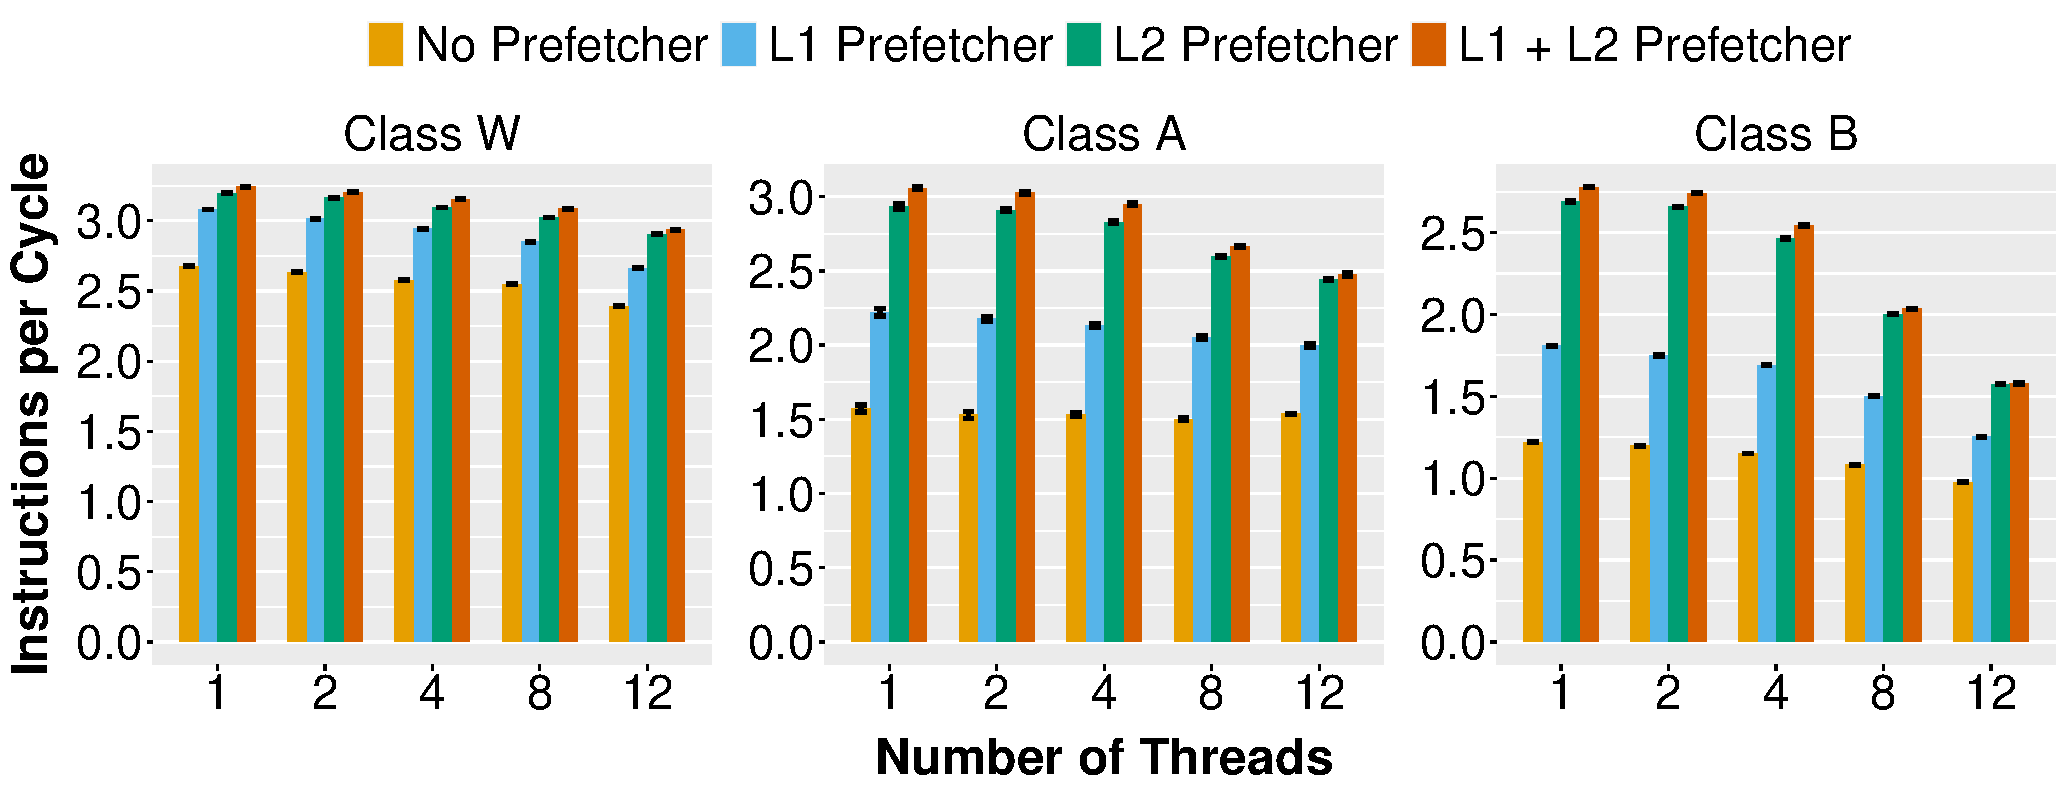
\includegraphics[width=\linewidth]{figures/fig6.pdf}
    \caption{IPC results of the NPB SP application, using input classes W, A, and B.}
    \label{fig:nas_wab}
\end{figure}





\begin{figure}[b]
    \centering
    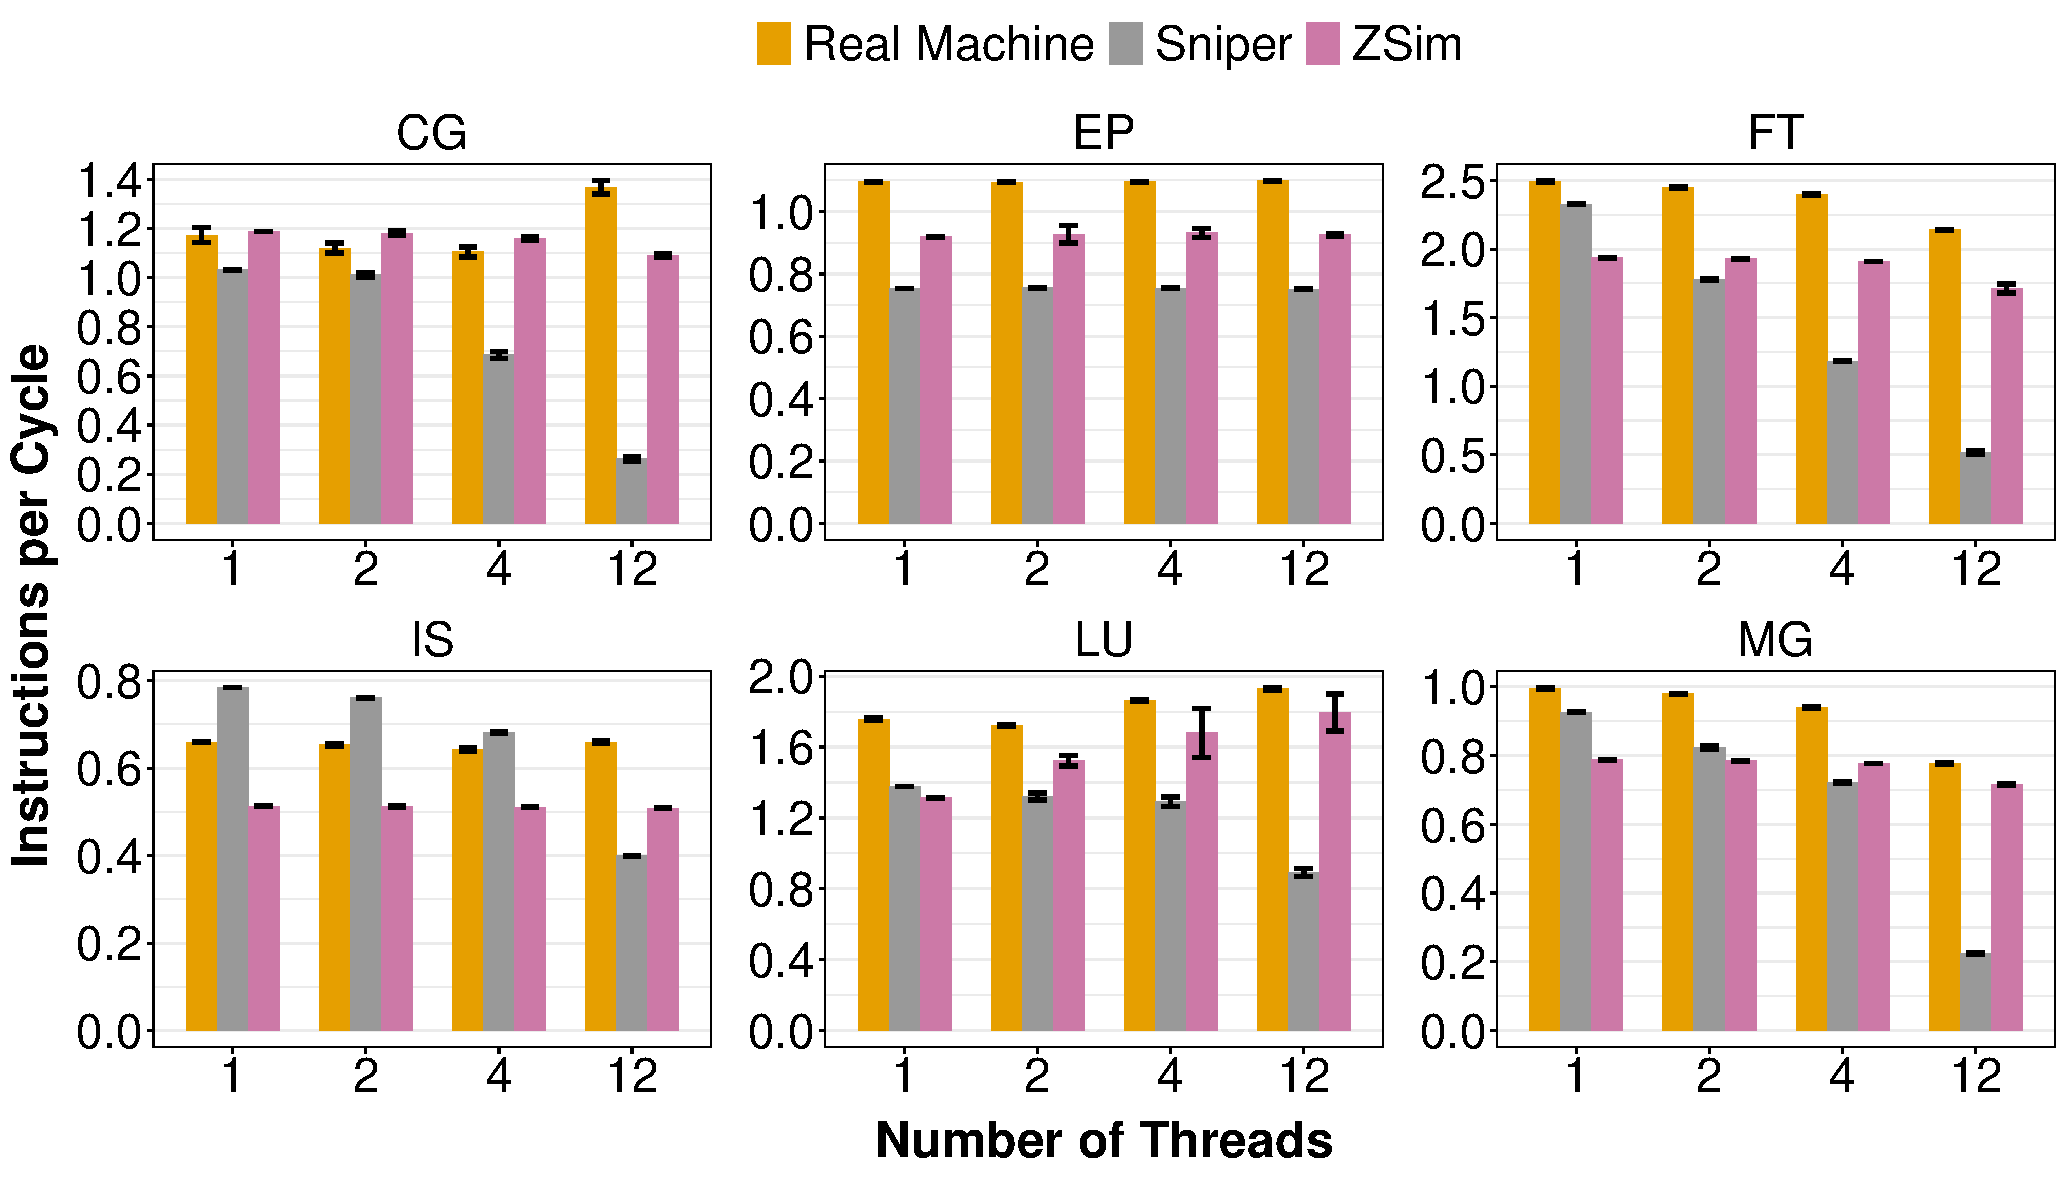
\includegraphics[width=\linewidth]{figures/fig8.pdf}
    \caption{Experimental results comparing the performance of simulation and real execution without prefetcher.}
    \label{fig:sims_nopref}
\end{figure}



\section{Investigating Prefetchers on Simulation}\label{sec:simulation}

As discussed in Section~\ref{sec:introduction}, parallel architecture simulation tools are necessary to develop and evaluate new techniques such as new prefetcher algorithms. In this regard, a key requirement is that these simulation tools can effectively simulate the parallel architecture and the parallel applications, bringing similar values of the metrics when compared to the real execution. In this section we therefore aim to clarify the following question: \textit{Using the ZSim and Sniper simulators, how do they behave and how accurately do they simulate NPB, accounting distinct prefetchers when possible?}

While simulators are a useful tool to test new architecture techniques, one drawback is the large amount of time that is often required by the simulations. For instance, the time to simulate the SP and BT applications of NPB using Sniper took more than one week. Sinuca~\cite{alves2015sinuca}, which is another parallel architecture simulator, took even more time to simulate, exceeding the maximum execution time allowed by our computing infrastructure. In this regard, we had to discard Sinuca from the study and with Sniper we simulated only a subset of the NPB applications, notably CG, EP, FT, IS, LU, and MG. 
We also only analyzed the simulation of prefetchers with the Sniper simulator, since ZSim does not simulate memory prefetchers. 



\begin{figure}[b]
    \centering
    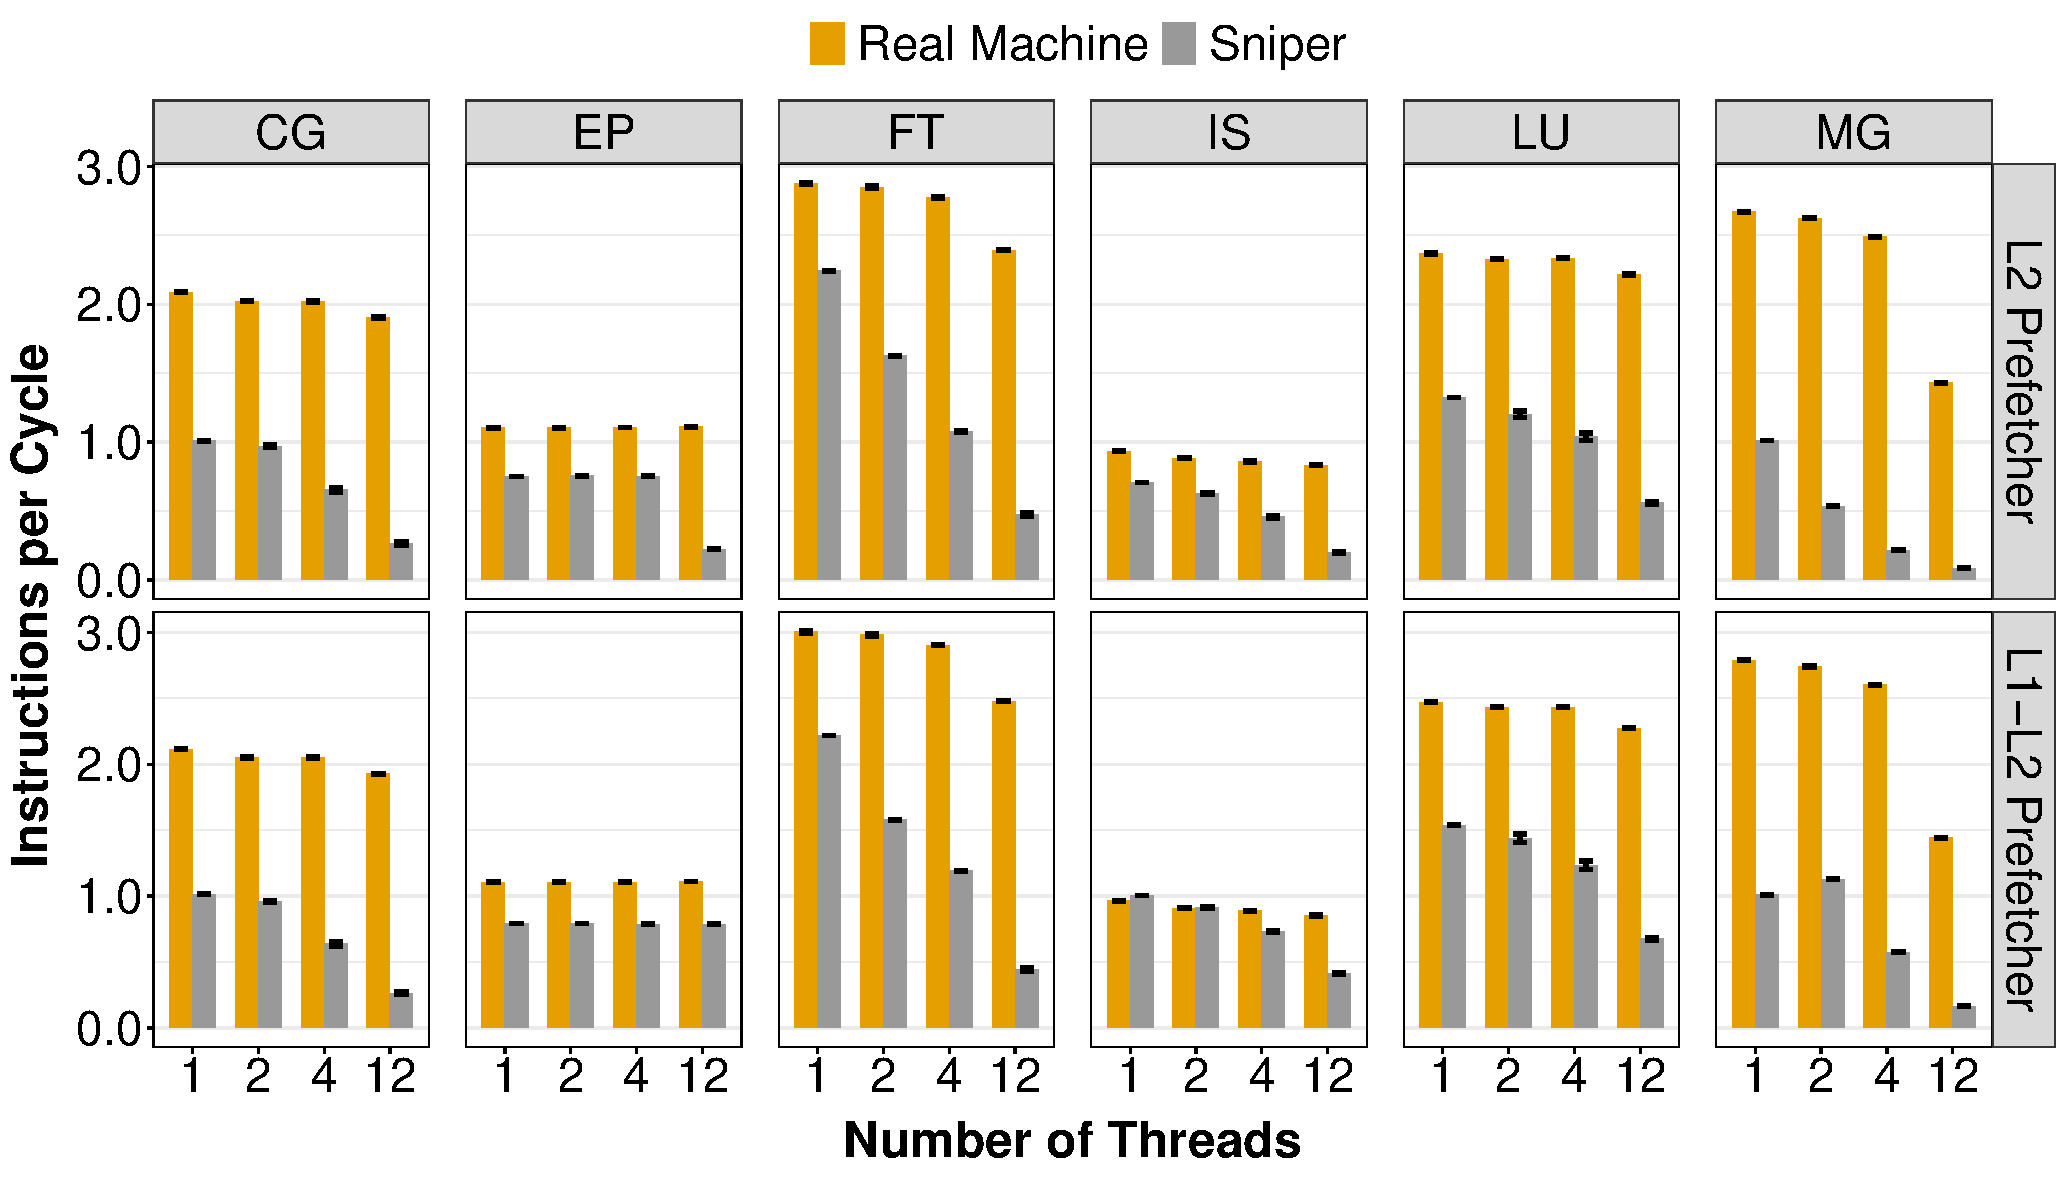
\includegraphics[width=\linewidth]{figures/fig88.pdf}
    \caption{Comparison of Sniper's L2 and L1+L2 prefetchers performance to the real executions results.}
    \label{fig:sniper_l2}
\end{figure}


Figure~\ref{fig:sims_nopref} shows the obtained IPCs when no prefetcher is used for six of the NPB applications, namely CG, EP, FT, IS, MG, and LU, simulating the input class A.
For that we disabled the prefetcher on both the real execution and the Sniper simulation. 
We did not make any specific changes to ZSim for this experiment, since ZSim does not support prefetcher simulation.



The only application where both simulators follow the real execution performance tendency is the EP. Since EP makes very little use of communication, it results in a simulation with very little contention events. 
This makes it easier for ZSim and Sniper to simulate EP, since simulating the effects of contention is arguably one of the most complex tasks in architecture simulation because of the out of order nature of contention events~\cite{sanchez2013zsim}.
However, for applications where communication and contention are more predominant, we can notice discrepancies between the simulation and the real execution. 
This discrepancy can be quite extreme. For instance, ZSim's MG simulation with 12 threads resulted in a average IPC 1.88 times higher than in the real execution, and Sniper's CG simulation with 12 threads resulted in an average IPC 4.6 times lower than in the real execution. 
The CG application is an interesting case because both Sniper and ZSim do not seem to accurately simulate the parallel CG execution (see Section~\ref{subs:cg}).
Both simulators predict a decrease in IPC as the number of threads increase, whereas in the real execution the trend is the opposite.




As aforementioned, accurately modeling contention is challenging. 
As mentioned in Section~\ref{ref:subs_zsim}, in ZSim's case it is assumed that most concurrent accesses happen to unrelated cache lines when considering small time scales. 
In that way, ZSim was engineered in such a way that requests to the same cache line may be simulated in a different order than the observed in the real execution~\cite{sanchez2013zsim}.
Therefore, the path of the data through the cache hierarchy may change, resulting in simulation inaccuracies.
This may explain the discrepancies of ZSim when simulating CG, as it is straightforward to devise that the concurrent and irregular memory accesses present in CG lead to concurrent accesses in same cache lines.
This same explanation can also be the case for the LU application, though a more detailed memory access analysis of LU is required to attest this argument.

As a general trend, for NPB applications with communication and contention, ZSim tends to underestimate the contention effects, while Sniper tends to overestimate the contention effects as the number of threads in the simulation increases.
For ZSim, this fact can be due to the above-mentioned design assumptions made during its development. 
For Sniper, in its turn, the reason can be more complicated, as it has been reported~\cite{carlson2014aeohmcm} that simulation errors in Sniper's memory model happen when simulating parallel applications with the interval model (see Section~\ref{subsubsec:sniper}). 





\textbf{In Figure~\ref{fig:sniper_l2}}, we compare the performance, in terms of IPC, of the Sniper's L2 prefetcher with the L2 prefetcher of the real machine, and the Sniper's L1+L2 prefetcher with the real counterpart, respetively.
In all evaluated NPB applications, we can notice discrepancies between the Sniper simulation results and the real machine results, with Sniper mostly underestimating the IPC performance, and overestimating the communication and contention effects with increasing number of threads.
Many reasons can explain this fact. 
First, as mentioned above, Sniper presents errors in its memory model when simulating parallel applications, even without considering prefetcher. 
These errors may be further amplified by adding a memory prefetcher in the simulation. 
Second, Global History Buffer (GHB)~\cite{nesbit2004data} L2 prefetcher implemented in Sniper differs from the Skylake's Stream~\cite{intelmanual} L2 prefetcher. 
In this regard, the GHB prefetcher offered by Sniper may not be suited to simulate Skylake. 
Modeling prefetcher algorithms with the same level of specificity of the real algorithms may be unfeasible, unfortunately, since manufaturers need to conceal key characteristics of their products (including prefetcher algorithms) in order to stay competitive.
\new{Another point worth noting is that, as mentioned in Section~\ref{subsec:exp-setup}, Skylake implements a non-inclusive L3 cache.
This non-inclusive L3 adds new complexity to the memory subsystem simulation since the data's location in this new organization depends upon several aspects~\cite{intelmanual}.}
Similarly to other architecture simulators, Sniper implements an inclusive L3 cache. This difference can also contribute to the discrepancies between the real execution using Skylake and the Sniper simulation.




\begin{figure}[b]
    \centering
    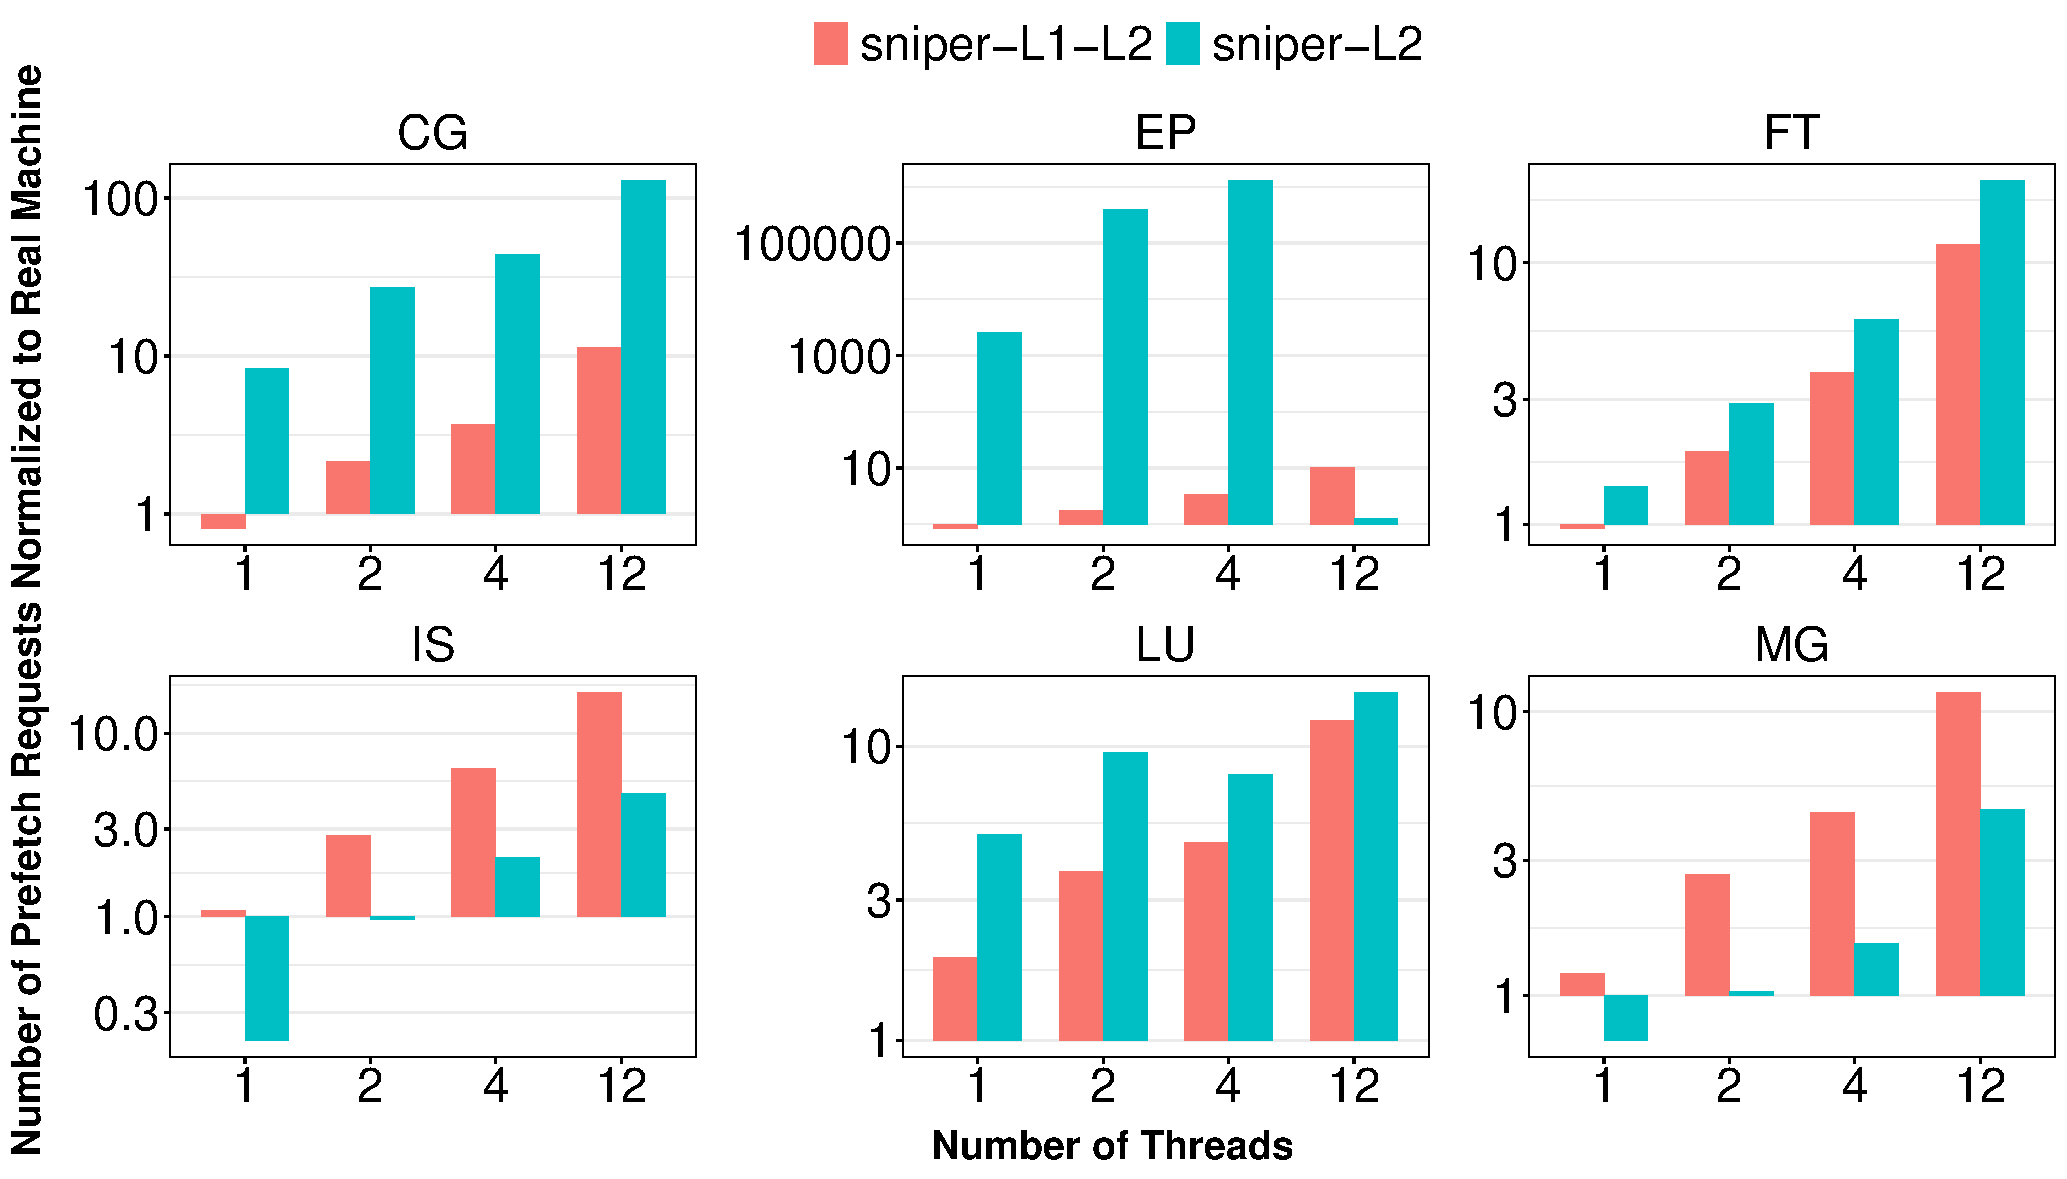
\includegraphics[width=\linewidth]{figures/fig99.pdf}
    \caption{Total number of prefetches issued by the simulation and by the real hardware (log scale on $y$ axis).}
    \label{fig:sniper_l2-rqsts-all-pf}
\end{figure}


In Figure~\ref{fig:sniper_l2-rqsts-all-pf} we present the total number of prefetch requests performed by the Sniper's L1+L2 prefetcher, the Sniper's L2 prefetcher, and their real counterparts. The number of prefetch requests for the L1+L2 prefetcher counts the prefetches on both L1 and L2 caches.
As expected at this point, Sniper's L2 prefetcher model was not capable to accurately simulate the Skylake's L2 prefetcher on the number of prefetch requests as well, presenting large discrepancies (notice the log scale on the $y$ axis of Figure~\ref{fig:sniper_l2-rqsts-all-pf}).
Sniper's L1+L2 prefetcher presented a total number of prefetch requests closer to the real execution. 
However, the similar number of prefetch requests of the Sniper's L1+L2 prefetchers does not translate in similar estimations of the applications performance, as shown in Figure~\ref{fig:sniper_l2}.
This may be due to the fact that the prefetches performed by Sniper are different in terms of usefullness. 
To attest this argument, in Figure~\ref{fig:sniper_useless_pf_ratio} we show the mean percentage of prefetches that were not useful during the executions in the real machine and in the Sniper simulation.
We can notice that the only application that sniper managed to accurately simulate the usefullness of the prefetches is the FT application.
When simulating the other applications with Sniper, Sniper considered the majority of prefetch requests as useless, with useless prefetches close to 100\% in some cases. 
This may indicate that Sniper's memory simulation module is having issues on simulating how the prefetched data is interacting with cache hierarchy. 
The non-inclusive L3 cache may also be a cause of this issue, since again Sniper considers an inclusive L3 cache.





\begin{figure}
    \centering
    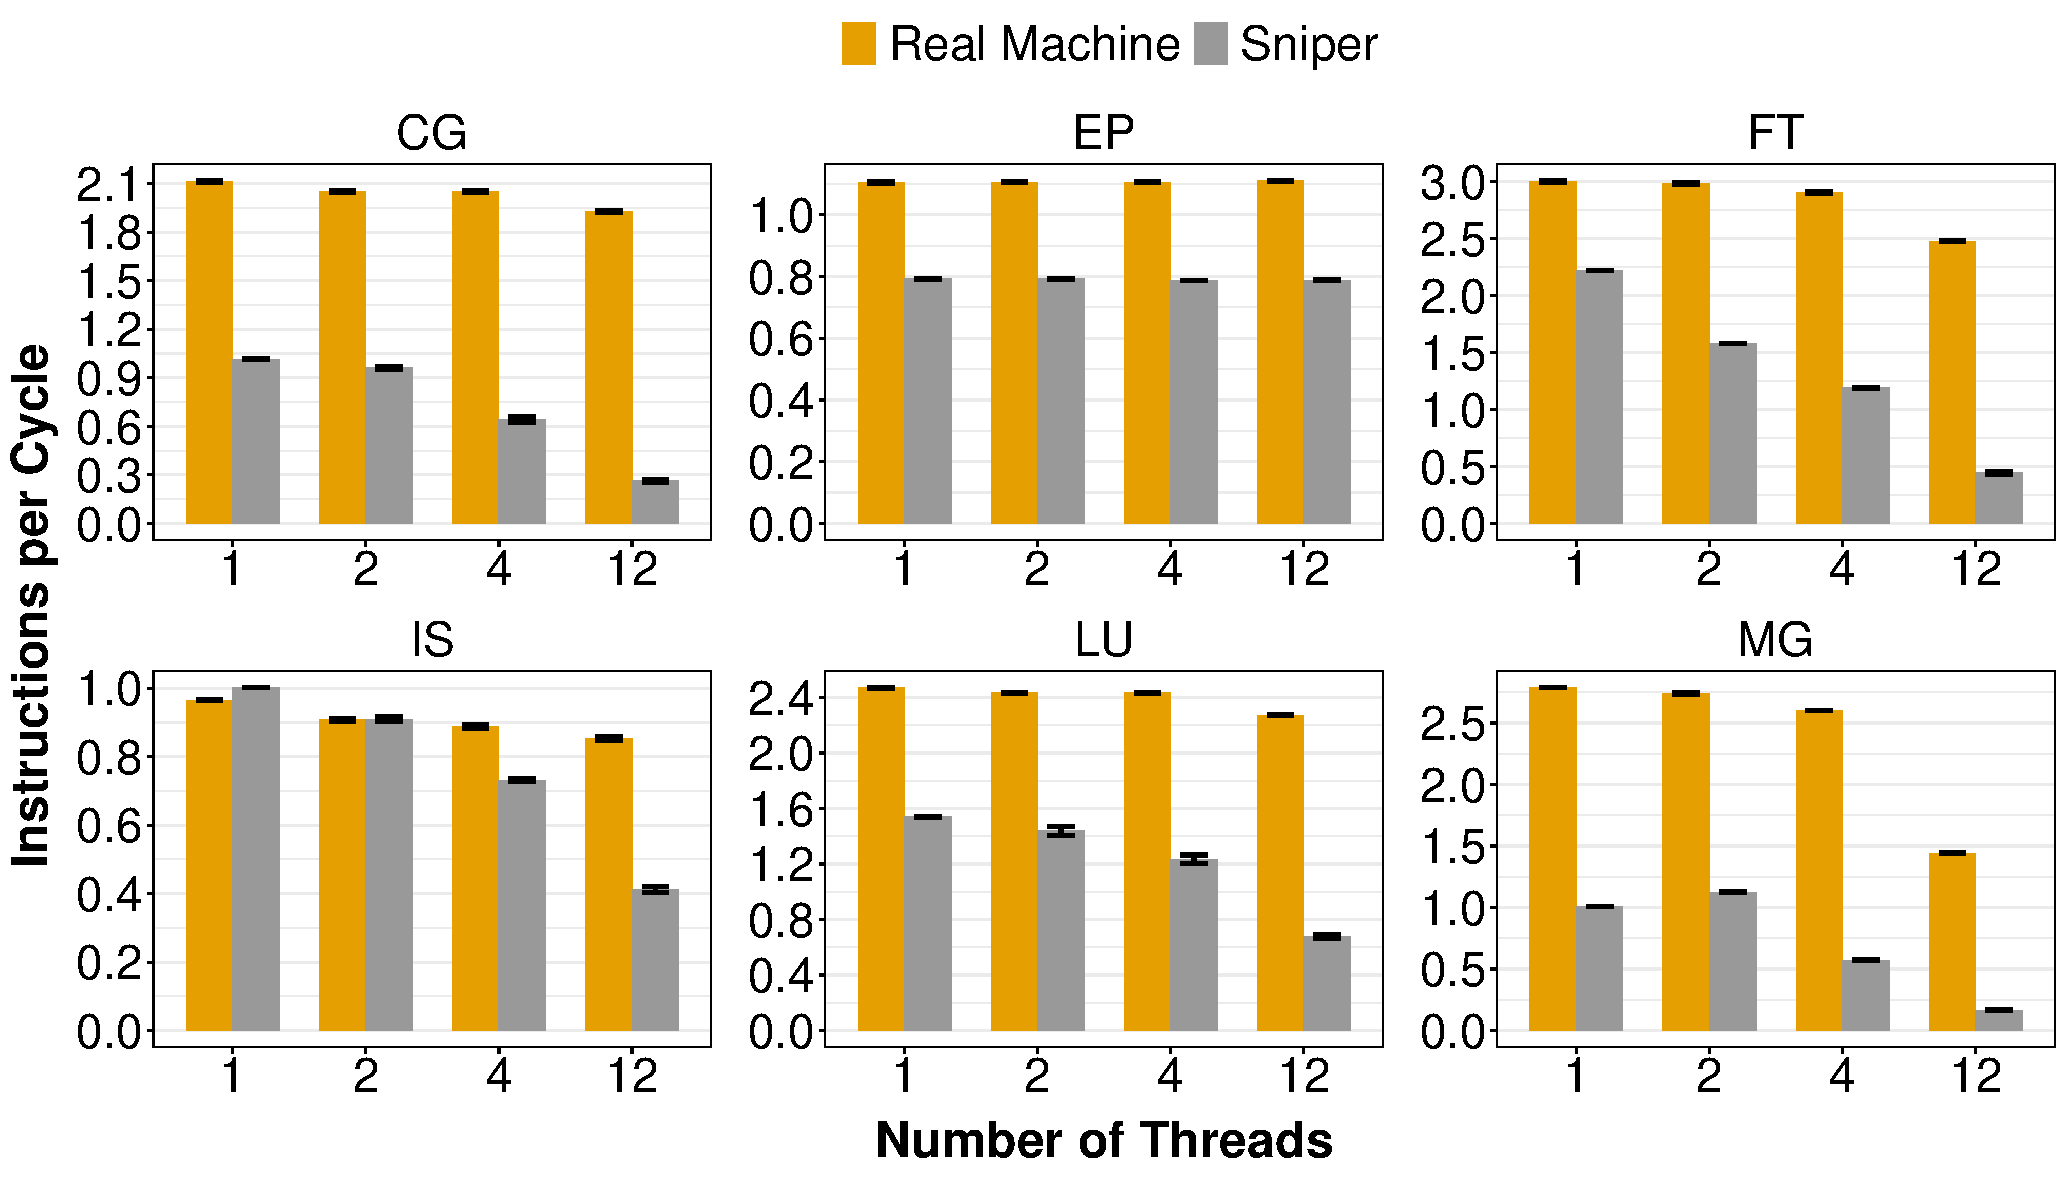
\includegraphics[width=\linewidth]{figures/fig10.pdf}
    \caption{Useless prefeteches performed by the simulation and by the real hardware, in ratio of the total number of prefetches.}
    \label{fig:sniper_useless_pf_ratio}
\end{figure}





\section{Discussion and Guidelines}\label{sec:insights}

An important aspect highlighted throughout the entire work is the difficulty of working with the memory subsystem, with the prefetcher and its algorithms being a special case.
The obscurity and confidentiality around the real implementation makes accurate models and algorithms impossible to be reproduced in simulators; moreover, for the same reasons above, simulator users have difficulties even in finding the proper parameters for the prefetcher models.


Regarding the observations we made in the experiments, we found several interesting characteristics in the studied prefetchers that may direct future works.
We have discussed how the L1 data prefetcher snooping the L1 cache requests can create contention by occupying the limited line fill buffers in the L1 cache.
Moreover, the interaction between the L1 prefetcher and the L2 prefetcher makes architecture studies that consider prefetchers harder to interpret.
Analyzing applications' performance, therefore, becomes harder due to the lack of control over the prefetchers and their implementations.

We argue that the use of both prefetchers (L1+L2) does not necessarily warrant significant performance gains, which is not intuitive.
When considering the L2 prefetcher, we obtained performance gains similar to when using both prefetchers, with the advantages of having more control over the experiments and the noise in the memory subsystem, faster simulation time, and thus less energy consumption due to the smaller number of \new{prefetch} requests being performed. 
This is comprehensible, as the current cache memory technologies allow a small difference in latency between the L1 and L2 caches, and \new{avoiding accesses to} the L3 cache becomes more critical in terms of latency.
\new{The access latency to the off-chip L3 cache memory is considerably higher than the access latency of the L2 cache (on average 7x, due to the mesh topology necessary to fully utilize the cache, as it is distributed in L3 off-core banks).}
Therefore, we advise using the L2 prefetcher as a standalone instead of both prefetchers (which is the default setting).
The L2 prefetcher observes the more relevant access patterns, as it prefetches data that would always require an access to the L3, thus hiding the large L3 latency.


With the increase in application parallelism, the execution time naturally becomes smaller. 
However, we see that the performance per core decreases as we increase the level of parallelism, showing the impact of memory accesses and communication over the application's performance.
As the amount of communication increases, the contention for the shared resources (interconnection network and LLC banks) increases as well.
Thereby, the request buffers of the caches and main memory become full, and the prefetcher cannot sufficiently mitigate the memory latency, resulting in small IPC values.
Thus, analyzing the communication pattern of applications is an important task to improve their performance, as applications which exert heavy memory pressure or communicate often can diminish the usefulness of a prefetcher.

\subsection{Considerations About the Prefetcher's Usefulness Degradation}
\label{subsec:pref_usefulness_thoughts}
Some practitioners have experienced this degradation of the prefetcher's usefulness in other applications, such as the experiences reported by Dell~\cite{SAPguide}, which claim 8\% increased performance for the SAP NetWeaver Portal application when disabling the hardware prefetchers.
In recent years, Intel implemented forms of reducing the prefetcher aggressiveness due to multiple reports such as Dell's, in order to avoid performance degradation.
Our real execution results show that even with high parallelism, Intel's strategy works, as the prefetcher never loses performance compared to an execution without prefetchers.
However, it would be interesting to test this assumption with simultaneous multithreading.

Nevertheless, our research shows that computer architecture researchers should always implement a prefetcher aggressiveness attenuator in the simulator model, and test their new implementations on highly parallel applications which exert memory pressure and inter-core interference~\cite{ebrahimi2009coordinated}, so that the possible negative impacts of their design can be properly evaluated.


\subsection{Generalization to Other Applications}
\label{subsec:other_apps}

We generalized a set of application characteristics during our experimental investigation, so that the results observed during this work -- specially the degradation of the prefetcher's usefulness as the level of parallelism increases -- can also be applicable for other types of applications. 
One of the main characteristics is about if a parallel application is embarassingly parallel -- which, for text clarity, we abbreviate to \textit{EmbPar} -- or not. 
Our observations can be extended for (i) any non-EmbPar application, and for (ii) EmbPar applications with in-place memory operations. Many parallel applications are non-EmbPar since EmbPar preventing operations such as locking and synchronization are often required in parallel algorithms (e.g., parallel Map Reduce or Stochastic Gradient Descent). EmbPar applications with in-place memory operations are less common, such as the pseudo-random number generation performed by the EP application of NPB. Our observation's exceptions are EmbPar applications that operate over vectors/matrices, such as parallel vector sum or matrix multiplication. These applications do not suffer from contention caused by synchronization or locking and may benefit from prefetchers since the number of memory accesses of these applications is significant.


\subsection{Good Practices and Guidelines}
\label{subsec:practices_n_experiences}
In this section, we present a summary of the main scientific and technical findings that we experienced during this work's development. These findings are framed into a list of good practices and guidelines that we suggest for future research and development on memory prefetcher with parallel applications, with and without simulation.

\begin{itemize}
    \item One shall pay attention on how the profiling tool collects performance data. Some profiling tools (such as Perf~\cite{de2010new}) collect performance data in a system-wide manner. In this context, system processes may affect the profiling results. However, when evaluating the performance of applications individually, we are concerned with performance data application-wide. Such data can be collected, for instance, using PAPI~\cite{terpstra2010papi};
    
    \item One shall be careful if a certain architecture research (notably prefetcher research) relies on an evaluation/validation performed by architecture simulators. In our experience, architecture simulators did not accurately represent real architectures, specifically when we consider memory prefetcher and parallel applications. Improving simulators' accuracy is a concerning and essential matter for the future of architecture algorithms research;
    
    \item Research on prefetcher algorithms for the L2 cache seems more promising to yield significant performance improvements -- as opposed to prefetcher algorithms for the L1 cache -- since, in our experience, accessing the L3 cache was a larger detriment to performance, as opposed to accessing the L2 cache;
    
    \item For highly parallel applications (in the order of dozens of threads on a single machine, see Section~\ref{subsec:other_apps}), memory prefetchers may not be critical for the application's performance since, in our experience, the prefetchers' performance seems to be bound to the performance degradation caused by the parallel contention.
\end{itemize}




\section{Conclusion and Future Work}\label{sec:conclusion}

Memory prefetcher algorithms have been widely used in processors to mitigate the performance gap between the processors and the memory subsystem. Analyzing and developing new prefetcher algorithms is a notoriously challenging task, especially due to the complexities and obscurities behind computer architecture development.

Memory prefetcher research is mainly possible thanks to architecture simulators that attempt to model the highly complex (and sometimes obscure) interactions present in the hardware. When we account for parallel, High-Performance Computing (HPC) applications, understanding the prefetcher's contribution to performance, on both the real hardware and in the simulations, becomes an important matter. 

In this work we performed an experimental investigation of the prefetcher's role in the performance of parallel, High Performance Computing (HPC) applications. Our investigation included a pioneer study on the prefetcher's performance in a simulated environment, taking the Sniper simulator as an example. Several insights were obtained regarding methodological aspects, the behavior of the studied prefetcher models, and how researchers and end users should handle prefetchers, in a both real and simulated scenario. 


Among these insights, one can highlight: (i) prefetching from the L3 to L2 cache presents a more substantial contribution to performance, (ii) memory contention becomes a larger constraint in the performance as the level of parallelism increases, limiting the prefetcher's contribution, (iii) Skylake's parallel memory contention is poorly simulated by ZSim and Sniper, and (iv) Skylake's non-inclusive L3 cache hinders the accurate simulation of NPB with the Sniper's prefetchers.

Since we observed that some prefetcher combinations perform unnecessary costly DRAM accesses, it is perhaps relevant to evaluate how these inaccurate prefetch requests impact energy consumption. Therefore, for future work, we intend to analyze the prefetcher's impact on energy consumption and energy-delay product (EDP)~\cite{gonzalez1996edp}. For instance, the EDP may help us understand which prefetcher configurations are more suitable considering both energy efficiency and execution time.
%Since some prefetcher combinations are performing unnecessary costly DRAM accesses, it is relevant to evaluate how these inaccurate prefetch requests impact energy consumption.
%Metrics as energy-delay product (EDP)~\cite{gonzalez1996edp} may help us to understand which prefetcher configurations are more suitable considering both energy efficiency and execution time.



\section*{Acknowledgements}
This work has been partially supported by Petrobras (2016/00133-9, 2018/00263-5) and Green Cloud project (2016/2551-0000 488-9), from FAPERGS and CNPq, program PRONEX 12/2014. This study was financed in part by the Coordenação de Aperfeiçoamento de Pessoal de Nível Superior (CAPES) - Finance Code 001. Experiments presented in this paper were carried out using the PCAD infrastructure, \url{http://gppd-hpc.inf.ufrgs.br}, at INF/UFRGS.

\bibliography{2020-ccpe-valeria}

\end{document}